%%%%%%%%%%%%%%%%%%%%%%%%%%%%%%%%%%%%%%
% This is the name of the style file.
%%%%%%%%%%%%%%%%%%%%%%%%%%%%%%%%%%%%%%
%
% phd  -> for a PhD dissertation
% ms   -> for an MS thesis
% If both phd and ms are used then phd will overide.  If none are used,
% then ms will be active by default.
%
% cpyr -> generate a copyright page
% lof  -> generate List of Figures
% lot  -> generate List of Tables
\documentclass[ms,cpyr,lof,lot]{uathesis}
%
%%%%%%%%%%%%%%%%%%%%%%%%%%%%%%%%
% List of any packages you use.
%%%%%%%%%%%%%%%%%%%%%%%%%%%%%%%%
%

\usepackage[nounderscore]{syntax}
\usepackage{listings}
\usepackage{algorithm, algpseudocode}
\usepackage[linewidth=1pt]{mdframed}
\usepackage{setspace}
\usepackage{amsmath}
\usepackage{amssymb}
\usepackage{epsfig}
\usepackage{graphicx}
\usepackage{changebar}
\usepackage{url}
\usepackage{environ}
\usepackage{textcomp}
%\usepackage{inconsolata}

\lstdefinelanguage{steve}
{
	morecomment=[l][\textit]{//}
}

\lstset{
		language=steve,
		basicstyle=\ttfamily\singlespacing\small,
	    emph={layout, int, uint, decoder, extract, as, var, else, if, requires, exact_table,
	    event, output, decode, goto, advance, drop, flood, set, write, clear, raise, insert, 
	    into, remove, from, match, case, while, miss, break, continue, Port, return, def},
	    emph=[2]{ start, in\_port, in\_phys\_port, egress, reflow, controller, all, timeout },
	    emph=[3]{ Error },
	    emphstyle={\color{blue}\textbf},
	    emphstyle=[2]{\color{green}\textbf},
	    emphstyle=[3]{\color{red}},
	    frame=single,
	    tabsize=2
}

%%%%%%%%%%%%%%%%%%%%%%%%%%%%%%%%%%
%%   Dealing with grammar style

\renewcommand{\syntleft}{$\langle$\ttfamily\itshape}
\renewcommand{\syntright}{$\rangle$}

\renewcommand{\litleft}{\ttfamily}
\renewcommand{\litright}{}

%\renewcommand{\ulitleft}{\ttfamily}
%\renewcommand{\ulitright}{}

%%%%%%%%%%%%%%%%%%%%%%%%%%%%%%%%%%%%

\graphicspath{ {./images/} }

\newlength{\currentparskip}
\newenvironment{minip}
  {\noindent
   \begin{minipage}{\textwidth}\begin{flushleft}
   \singlespace
  }
  {\end{flushleft}\end{minipage}\vspace{\baselineskip}}

\setlength{\grammarparsep}{1pt}

%\noindent\begin{minipage}{\linewidth}
%\begin{grammar}
%\singlespace
%
%
%\end{grammar}
%\end{minipage}


%
%%%%%%%%%%%%%%%%%%%%%%%%%%%%%%%%%%
% List of definitions you define.
%%%%%%%%%%%%%%%%%%%%%%%%%%%%%%%%%%
%
\def\ds{\displaystyle}
\def\E{\epsilon}

%%%%%%%%%%%%%%%%%%%%
% Defining inline grammar macros
%%%%%%%%%%%%%%%%%%%%
\def\la{\textlangle{}}
\def\ra{\textrangle{}}
\def\mn{\text{-}}
\newcommand\grddd[4]{\la\textit{\texttt{#1}} \mn \textit{\texttt{#2}} \mn \textit{\texttt{#3}} \mn \textit{\texttt{#4}}\ra}
\newcommand\grdd[3]{\la\textit{\texttt{#1}} \mn \textit{\texttt{#2}} \mn \textit{\texttt{#3}}\ra}
\newcommand\grd[2]{\la\textit{\texttt{#1}} \mn \textit{\texttt{#2}}\ra}
\newcommand\gr[1]{\la\textit{\texttt{#1}}\ra}

%

\title{Steve - A Programming Language for Packet Processing}
\author{Hoang Nguyen}
\conferraldate{May}{2016}

%The following commands specify the names and titles of people that
%will appear on the signature page.
%
%These four will always be needed.
\advisor{Andrew Sutton}
\chair{Timothy O'Neil}
\collegedean{John Green}
\gradschdean{Chand Midha}
%
%For a PhD dissertation, specify a coadvisor and three committee
%members, or four committee members only.  For an MS thesis use either
%one coadvisor or one faculty reader, not both.
%
%Typical commands for a PhD dissertation (uncomment only 4).
%\coadvisor{Name of Coadvisor}
\committee{Name of 1st Comm Member}
\committee{Name of 2nd Comm Member}
\committee{Name of 3rd Comm Member}
\committee{Name of 4th Comm Member}
%
%Typical commands for an MS thesis (uncomment only 1).
%\coadvisor{Andrew Sutton}
\facreader{NAME 1}
\facreader{NAME 2}

\begin{document}
\maketitle
\chapter{INTRODUCTION} \label{ch:intro}

% FIXME: The introduction needs to flow. Don't break it up into this kind of
% question and answer dialog, and don't skimp on motivation. Take this guy's
% PhD thesis as an example:
%
% http://www.cs.colostate.edu/~christos/thesis/chp1.pdf
%
% It's a little more detailed than you'll need, but it's a good example of
% how to motivate the problem and organize both the solution and your
% contributions.

% FIXME: Use \emph to emphasize terms, not boldface.

% FIXME: Use this sentence in your abstract.

The Internet is nowadays ubiquitous with everyday life. In the last twenty years,
the industry has rapidly evolved to incorporate all kinds of new Internet services:
cloud services, web services, Internet of Things, etc. As the world grows
more reliant on services provided over a network, so must the network evolve.

Modern routers and switches provide the backbone for the Internet.
These modern devices implement two fundamental components in their firmware: the
\emph{control plane} and the \emph{data plane}.
The control plane decides where packets should be sent and is capable of learning
new forwarding behaviors. The control plane commands the data plane.
The data plane is responsible for moving packets between ports.
Over time this conventional type of networking has become too rigid, unscalable, and
proprietary to support evolving technologies. 

Defining network functionality in firmware is inherently inflexible.
Firmware is architecture-dependent, difficult to write, and challenging to update
regularly.
Conventional switches are unscalable because they must deal with most or all
common protocol headers.
With dozens of common protocols now, and potentially dozens more in the future,
it becomes evident that this model cannot last forever.
Additionally, many devices are black boxes,
only exposing an interface designed by the vendor,
making them difficult to customize for enterprises with special needs.
Due to these issues and others,
a new paradigm for networking was created. 

This new paradigm
is called \textit{software-defined networking} (SDN). The Open Network
Foundation (ONF) defines SDN as ``the physical separation of the network control
plane from the forwarding [data] plane'' \cite{onf_sdn_def}.
The control plane is removed from the firmware.
Instead, it is implemented in software which typically runs on a separate machine.
This software control plane is capable of controlling several devices over a
single network using messages.
The most popular open-source standard for this type of networking is OpenFlow \cite{openflow_spec}.

This programmable control plane gives programmers the ability to
provide network functions (such as firewalls, network address translation, etc) in 
software rather than proprietary hardware.
Any programmer can write regular software for common operating
systems and processors to control the behavior of their networking device.

The programmable control plane is only the first step. The next
step is the \emph{programmable data plane}. By decoupling the data and control planes, 
it allows them both to evolve separately. A programmable data plane provides
two key benefits that the software control plane cannot: low-latency, customized packet processing and \emph{protocol independence}.

In the control and data plane relationship,
the control plane is smart but slow, while the data plane is fast yet dumb. That is,
the control plane can perform general purpose computing but communicating with
it has high latency. The data plane, on the other hand, is the fast path for packet processing.
It has very limited computing power, but can process packets at a low latency.
As programmable data planes evolve and support more flexible instruction sets,
communicating with the control plane becomes less necessary.

Protocol independence means that a networking device is not required to support
a suite of well-known protocols (ethernet, IPv4, TCP, etc) by default.
Rather than relying on specialized hardware or firmware tailored towards parsing/decoding
these protocols, the data plane supports processors
and generic instructions that a user could use to decode and operate on
any header and field.
This allows users to define their own protocols in addition to
supporting well-known protocols. This makes the data plane scalable, that is, it
can adapt to new headers easily.

In order to pursue programmable SDN devices, there must be a language to write
packet processing programs. A number of language solutions arise here.
Some attempt to solve this problem by providing APIs for existing programming languages
(specifically C/C++).
Others attempt to produce domain-specific languages (DSLs) for SDN devices.
The focus of this thesis is one such DSL, Steve, a language for the safe and
efficient specification of packet processing applications for programmable data planes.

% Packet processing and forwarding logic is usually performed using an abstract
% model known as a \emph{packet processing pipeline} which is a generalization of
% the pipeline model described by OpenFlow \cite{openflow_spec}.


%
% The programmer can customize a switch with customized packet processing
% applications and forwarding rules. Typically, this is done through an abstract
% model called a \textit{packet processing pipeline}.
% The pipeline makes decisions, performs operations, and applies forwarding rules on packets.
%
% Forwarding rules can handle any header and can be user-defined. It opens the way
% to networking applications made for custom protocols and forwarding behaviors.
% By changing the program which drives the packet processing pipeline, the user
% can \textit{change the device's behavior without changing the device's
% hardware}. The same device can go from being a repeating hub to a MAC learning
% switch to a router just by running a different program on it.

\section{The Steve Programming Language}

Steve is a protocol independent, architecture independent, strongly-typed,
declarative language for writing packet processing applications on SDN devices.
Steve allows programmers to define network functions using an abstract model
known as a \emph{packet processing pipeline} -- a generalization
of the pipeline defined by OpenFlow \cite{openflow_spec}.
A packet processing pipeline is an algorithm that
uses multiple stages to process and forward packets.
Steve provides high-level language features for specifying this pipeline.
Specifically, Steve allows for the definition of:

\textbf{Header Structures}.
A programmer may define the structure of any protocol header using an abstract
mechanism known as a \emph{layout}.
A layout specifies what fields are in a header, the lengths of those fields,
and types for those fields.

\textbf{Decoders}. Decoders are special functions for extracting fields from a
packet header. They conform to user-defined layouts, making them flexible enough
to deal with any protocol header.

%
% Steve allows the user to program special functions decoders
% which are used for decoding and extract fields from a header. Decoders allow the
% user to specify which fields they need. Decoders do not require that a user
% extract all fields if they do not need those fields. The user is not required to
% manually extract the bytes associated with a field. Instead, the user gives a
% field name from the header layout they defined, and the language generates the
% code for them.

\textbf{Flow tables}. 
In networking, a \emph{flow} is a group of packets from a source to one or more 
destinations. In order to facilitate these flows, Steve uses the
\emph{flow table} (an OpenFlow inspired abstraction). 
A flow table is a dynamic
decision table which classifies packets into groups (flows) using
decision rules (known as \emph{flow entries}).
Packets which are part of the same flow have a common set of \emph{actions}
applied to them.
Flow tables are responsible for the majority of forwarding logic.

\textbf{Actions}. Actions provide a way to modify a packet's fields, add/remove
flow entries from tables, and forward/drop packets. Steve actions are a generalization
of OpenFlow's instructions and actions.

\textbf{Pipeline Composition}. A Steve pipeline is a composition of two kinds of stages:
decoders and flow tables.
A packet moves through these stages which perform some set of processing operations.
Eventually one of these stages will make a forwarding decision for that packet.
The language provides a mechanism for connecting these
stages together in a number of flexible ways.

\textbf{Event handling}. The pipeline may raise events when it cannot handle a
packet. Event handlers may be defined to deal with events such as learning a new
flow, removing an old flow, etc.

Though Steve is an SDN language, it also supports a number of general purpose
features similar to C. Steve supports functions, variables, arithmetic, branching, looping
and a foreign function interface which may be used to call linked C functions.

\section{Motivation: Issues with Low-level Languages}

A network program must enforce safety over any other concepts.
Network programs, especially those running on high-traffic devices, must not
crash due to logical mistakes or unnoticed undefined behaviors.
Such errors could result in security holes, denial of service attacks, and
disastrous network downtime.

Typical packet processing programs are written in low-level languages, most
commonly C. These C programs usually work with data plane programming APIs such
as Open Data Plane (ODP) \cite{odp_webpage} and the Data Plane Programming Kit
(DPDK) \cite{dpdk_webpage}. Programming network functions in C can be prone
to logical error and unnoticed undefined behavior stemming from buffer management
and resource management. These issues are compounded by the fact C is a general
purpose language not tailored towards packet processing, thus the burden of safety
is left to the programmer.
Specifically, C programs open the opportunity for logical errors and undefined
behaviors such as:

\begin{itemize}
\item accessing memory outside the bounds of a packet buffer or within a constrained
region of memory,

\item writing bytes which exceed a constrained subset of the packet
resulting in a buffer overflow (i.e. writing new bytes into a header field
but exceeding the size of that field),

\item buffer underflow resulting from not writing enough bytes when modifying
a field,

\item using the value of a field in an operation that is not supported by its
range of value,

\item non-terminating cycles in program logic (an infinite loop
triggered by a single packet),

\item incorrect assumptions about decoding state. That is, a programmer using
a field which they have not extracted yet.
\end{itemize}

Programmers using C for SDN applications are also burdened with management of
device resources. Specifically, a C programmer must manage:

\begin{itemize}
\item memory. The programmer must manage their own buffers for holding packet
data and packet meta data. This opens the opportunity for accidental
memory leakage.

\item ports. The programmer is responsible for receiving, reading, and forwarding
through ports. This process should be decoupled from the packet processing logic
for modularity. A packet processing application should be architecture independent
whereas port management is a architecture dependent problem.
\end{itemize}

% Low-level packet processing code can be very light on easy to understand
% abstraction and very heavy on gritty implementation details. The programmer
% should be focusing on high-level abstractions; concepts such as: what fields are
% needed, what operations must be performed on these fields, conditional decision
% making, packet classification, etc. Instead, they are worried about the many
% common ailments of writing in low-level code.
%
% The programmer must deal with resource allocation and management. They must deal
% with allocating their own buffers for storing packets and by extension must deal
% with de-allocating those buffers. This type of resource management is prone to
% accidental memory leakage, especially in C. Memory leakage of gigabytes of data
% will quickly bring a system down.
%
% The programmer must directly manage ports. They are also responsible for
% manually receiving, reading, and sending packets on those ports. This is code is
% common to all packet processing applications. The programmer should not be
% burdened with this kind of common code when writing a packet processor.
%
% When working with packet headers, the programmer must manually work with raw
% arrays of bytes. The burden of decoding fields from byte arrays and interpreting
% the value of those fields is shifted onto the programmer. Manual decoding can be
% a painful process on its own. It is prone to error, particularly off-by-N
% errors. When reinterpreting those bytes into header data structures, the result
% can be disastrous if the bytes are wrong or the data structure is wrong. Moving
% or copying those bytes around is particularly prone to buffer overflows.
%
% A number of other common problems come up when working in low-level code.
% Undefined behavior from reading past the end of packet buffers can be one.
% Performing operations on null pointers, invalid pointers, or uninitialized
% memory is another.
%
% Steve and its runtime, Flowpath, attempt to remedy most of these problems. The
% objective is to abstract many of these low-level details. Instead, the
% programmer only focuses on the high-level abstractions. Specifically, the Steve
% language focuses the programmer on writing the packet processing pipeline and
% makes the grittier details opaque.

\section{Contribution: A Language for Defining Safe Pipelines}

The Steve language provides a type and constraints system to ensure the safety
of all Steve-defined packet operations and pipelines.
Steve targets the runtime environment, Flowpath, abstracts the resources
such as memory and ports, of a given hardware device so the Steve program does not
have to.
In addition, Steve uses an optimizing compiler to ensure efficient code generation.

\subsection{Type Safety}

Steve is a statically-typed language. The compiler performs additional work to
enforce strict safety guarantees so that runtime checks can be avoided as much as possible.

The Steve type system ensures that operations on header fields are valid and
well-defined. 
To reduce errors related to working with fields as byte buffers, Steve allows
for the representation of fields as arbitrary precision, signed or unsigned integers.
Implicit integer conversions can be applied to these fields where necessary.
Conversions prevent field modification from ever underflowing or overflowing.

Steve does not support pointer types, meaning that the programmer is never
concerned with null or invalid pointer addresses. Instead, Steve supports reference
types which are guaranteed to refer to initialized memory.

%\begin{enumerate}
%\item the representation of fields as
%arbitrary precision, signed or unsigned integers, (as long as they
%are multiples of 8). This allows the programmer to avoid using arrays of bytes
%to represent fields.
%
%\item logical and arithmetic expressions which are type checked
%to ensure no undefined behavior happens (e.g. shifting by negative values,
%adding to a boolean, etc).
%
%\item implicit conversions can be applied where necessary (e.g. integer size
%promotion, unsigned to signed conversions, etc).
%
%\item buffer overflow/underflow prevention. 
%Writing a new value into a header field \textit{never} causes accidental
%buffer overflows. The Steve compiler uses implicit conversions to guarantee that
%the size of the new value fits exactly into the byte width of a field. If the
%new value is represented in less bytes than the size of field, it gets extended
%to fit. Values that are too large get truncated.
%\end{enumerate}


% Specifically, the Steve language aims to avoid:
%
% \begin{itemize}
% \item accessing memory outside the bounds of a packet buffer,
%
% \item writing bytes which exceed a contrained subset of the packet
% resulting in a buffer overflow (i.e. writing new bytes into a header field
% but exceeding the size of that field),
%
% \item buffer underflow resulting from not writing enough bytes when modifying
% a field,
%
% \item using the value of a field in an operation that is not supported by its
% range of value,
%
% \item non-terminating cycles of decoders and table matchings (an infinite loop
% of packet processing),
%
% \item incorrect assumptions about decoding state. That is, a programmer using
% a field which they have not extracted yet.
% \end{itemize}

\subsection{Pipeline Constraints System}

The Steve compiler ensures certain guarantees about the correctness of a Steve
pipeline. Steve pipelines may be represented as directed acyclic graphs. The
Steve compiler performs analysis on this graph to enforce the following
constraints.

\begin{enumerate}
\item Fields that have not been extracted by a decoder cannot be used. 

\item The traversal of a packet through a pipeline is always a linear
progression. That is, a packet may never enter a non-terminating cycle
of decoders and tables.
\end{enumerate}

\subsection{Resource Safety}

Steve never requires the user to heap allocate resources. The majority of
allocation is done on the stack, ensuring Steve applications are free of
memory leakage and faster (as heap allocation tends to be slow).

Steve relies on its runtime system, Freeflow \cite{freeflow_software}, 
to manage system resources such as
ports, packet reading, and packet buffer allocations.
This decouples the logic of system resource management from the packet
processing logic.

\subsection{Efficiency}

%Steve's programmable decoders provide the user the chance at certain
%optimizations. Steve allows the user to specify exactly which fields from a
%header they want extracted rather than forcing them to extract the entire thing.

High-level abstractions tend to produce performance penalties in exchange
for safety. The Steve compiler tries to reduce this penalty as much as possible.
The Steve compiler generates LLVM intermediate representation (IR) code
\cite{llvm_webpage}. The LLVM IR optimizing compiler is able to produce 
code equivalent to C programs such as:
function inlining, peephole optimizations, etc.

Steve may also customize the LLVM compiler to produce
specialized instructions that are optimized for the architecture running
the application. This would be future work.

\section{Thesis Overview}

This thesis is organized as follows.

Chapter \ref{ch:pipeline_model} describes the components of Steve programs
and pipelines. It provides many of the abstract concepts a programmer must
understand about packet processing before they can begin writing a Steve
program.

Once a programmer understands the fundamentals of the pipeline processing model,
they may begin with the Steve tutorial in Chapter \ref{ch:tutorial}.
This tutorial explains how to write network applications using the
Steve programming language. Sample networking applications are also presented in
this chapter. These same samples are presented again in Appendix
\ref{ap:steve_programs}. 

Chapter \ref{ch:users_guide} serves as a reference
manual which includes semantic, grammar, and typing rules for the language.
This reference manual may be helpful to refer to when confused about a
Steve code example.
It is not to be read as a typical chapter. Instead, one should 
treat it like an annotated appendix.

Chapter \ref{ch:flowpath} describes how Steve and its runtime environment, Freeflow,
interact with each other and the underlying hardware system.

Chapter \ref{ch:experiments} provides experiments using sample Steve
applications. Pcap files are run through Steve applications to measure the data
rate and raw packet rate that each application is capable of running at on a
Linux machine.

Chapter \ref{ch:related} describes similar
works in the field of SDN and SDN programming languages. It also provides a
background into SDN and the different approaches Steve takes to other languages
of its kind.

\chapter{RELATED WORKS} \label{ch:related}

\section{Freeflow} \label{rel:freeflow}

Freeflow is a highly programmable, protocol oblivious data plane being developed
by Flowgrammable \footnote{https://github.com/flowgrammable/freeflow/}. Steve is
designed to program the Freeflow data plane and generates code targeting its
Flowpath runtime environment. Freeflow adopts a component model similar to an OpenFlow switch. A basic OpenFlow switch
has three major components: a packet processing pipeline, ports, and a channel
to an external controller application \cite{openflow_spec}. A Freeflow data
plane loads Steve applications which control the logic behind the packet
processing pipeline.

\section{OpenFlow} \label{rel:openflow}

An OpenFlow pipeline is defined as a sequence
of one or more \textit{flow tables} and a \textit{group table} which handle
packet lookups, decision making, and forwarding \cite{openflow_spec}. Steve's packet processing pipeline differs from the traditional OpenFlow
semantics in a number of ways. First,
Steve provides language features for a user to create flow tables and define
their flow entries, but does not yet support group tables. 

Second, a Steve pipeline has more than \textit{just} flow tables. Steve
pipelines will also have \textit{decoders} which may be interleaved between
tables. Decoders define how fields get decoded (or parsed) and extracted. In
most switches, decoding is handled by specialized hardware that deal with
well-known headers. OpenFlow only supports certain fields from these headers,
known as OXM fields \cite{openflow_spec}. However, the Freeflow data plane is
protocol oblivious, knowing nothing about any specific headers; therefore
decoding must be an explicit user-defined stage of the pipeline. By extension,
Steve does not, by default, support these OXM fields either.

Third, the semantics for packet handling using an external controller are different. An OpenFlow controller is software used to control an OpenFlow switch \cite{openflow_spec}. It will handle "exceptional events" such as inserting,
removing, and updating flow entries or processing packets which the pipeline
could not. However, Steve and Freeflow do not use nor expect an external
OpenFlow controller nor do they use OpenFlow messages to communicate with that
controller. 

Steve and Freeflow attempt to reduce the role of the controller. Controller
functions, which would typically handle exceptional cases (such as table
manipulation and un-handled packets), can be written in Steve using special
"event" handlers functions. These event handlers are executed by the data plane
on a special internal Freeflow "controller" thread rather than relying on an
external controller. 

\section{SDN Data Plane Configuration Languages} \label{rel:p4}

Steve is a language for modifying the packet processing and forwarding functionality of a data plane. Steve is \textit{protocol oblivious}, meaning it does not by default
know of any well-known network protocols (IPv4, IPv6, TCP, etc). Instead, it
provides language features for programmers to deal with any protocol, making the
language more scalable for future protocols. Other SDN languages are pursuing
these idea as well.

The P4 language \cite{p4_spec, p4_spec2} is another high-level language for
defining protocol oblivious packet processing pipelines. It is probably the
most widely adopted SDN language. P4 allows users to define packet headers,
packet parsers and
match+action tables (which are equivalent to OpenFlow flow tables). Parsers are
used to extract entire headers and store them in a "parsed representation"
before entering pipeline processing. When the packet enters the pipeline,
match+action tables match against fields in the parsed representation and
perform actions on matched packets. 

Protocol-Oblivious Forwarding (POF) \cite{pof_fis, pof, pof_impl} is another
project also tackling the problem of protocol oblivious pipeline processing. POF
is a very low-level, assembly-like, instruction set. The POF instruction
set gives the programmer very fine-grained control of which fields get parsed.
The POF programming model uses metadata as a "scratch pad" for parsing fields,
requiring that the
programmer represent fields as generic \{offset, length\} pairs, known as
"search keys" \cite{pof}. When performing table matching, a programmer specifies
an array of these search keys to match against the flow table \cite{pof_impl}.
Essentially, fields only get extracted as they are needed, right before matching
against a given table.

POF also supports additional actions that allow the data plane to manipulate
flow tables \cite{pof}. This includes adding, removing, and updating flow
entries. Though these actions are traditionally left up to the controller, they
are useful because they reduce the load on the controller and provide
flexibility to the data plane. This feature is notably absent from other SDN
languages.

The POF instruction set is difficult to write in and does not have the safety
guarantees of a higher level language. The programmer is burdened with the
error-prone task of parsing by manually specifying which bits comprise a fields. 
A high level language compiling into POF instructions would thus be ideal.

Steve tries to take the best of both worlds. Steve can define decoding functions
similar to P4 parsers, with the added benefit of allowing the programmer to only
extract the fields they need, reducing the amount of time needed to parse
overall. The \{offset, length\} pairs describing each field get generated by the
Steve compiler rather than being manually written by the programmer, thus
reducing
the risk for error. Steve decoders may also be interleaved between tables,
meaning fields can be extracted, as needed, right before table matching like
POF. Like P4,
Steve decoding can also happen all at once "up-front," before any table
matching. 
It is up to the programmer to decide which is better. This makes Steve
decoders a little more robust than either P4 or POF. 

Steve supports high-level definition of flow tables (or match+action tables in
P4). Additionally, Steve also allows the programmer to define flow entries. This
means the match field values and actions for each flow entry can be expressed
within the language, allowing the Steve compiler to ensure safety and
correctness guarantees over them. For example, adding a flow entry that causes
an infinite loop is always prevented. This task is normally left up to the
controller during runtime, which can be slow. Steve also supports instructions
for adding and removing these flow entries from tables like POF.

Unlike P4 and POF, Steve is not \textit{just} an SDN specific language; it is an
extension to a general purpose language. It thus supports features like
functions, function calls, lexical scoping, loops, conditional statements, and
local/global variables. Steve also has support for types, arithmetic
expressions, and comparison expressions. On top of that, it automatically links
against the C Runtime Library, supports calls to external functions, and may be
statically or dynamically linked against any library.

Admittedly, P4 is a more mature language than Steve. P4 supports things like
meters, variable sized fields, table matching methods (Steve only supports exact
matching), and certain actions that Steve does not. P4 can also target more
platforms than Steve, which currently only compiles into modules for Freeflow.
POF also supports certain actions and table matching methods that Steve does not
currently support.

NetASM is an intermediate representation language for programmable data planes
\cite{shahbaz2015netasm}. It aims to solve the same issues as POF, but also provides a language that is target/device independent. The goal is for higher level languages to compile into NetASM which can then be compiled into platform-specific code by device-specific compilers.

\section{Other Languages} \label{rel:frenetic}

Other languages are protocol-dependent and are designed to program the control plane. The Frenetic project has produced a family of network programming
languages. The Frenetic language is a declarative language, embedded in Python,
that uses SQL-like queries to classify packets and a library for describing
packet forwarding policies over a collection of network switches
\cite{foster2011frenetic, foster2013frenetic}. This language is designed to
abstract away the difficulties of programming a centralized SDN controller. Its
sister project, Pyretic, does the same with some divergence in how forwarding
policies are expressed \cite{modularpyretic}. Both languages try to confirm the correctness of a program over an entire network.

NetCore is a network programming language for expressing forwarding policies and
generating classifiers from those policies \cite{monsanto2012netcore}. These
classifiers then get installed on switches. NetKAT is a language, inspired by
NetCore, for expressing packet processing functions and reasoning about a
network using Kleene Algebra \cite{kozen2014netkat, anderson2014netkat}. NetKAT
attempts to prove the correctness of its network programs through mathematical theory.

\chapter{THE PACKET PIPELINE PROCESSING MODEL} \label{ch:pipeline_model}

Steve uses a \textit{pipeline processing model} to process packets. The pipeline processing model is a series of \textit{data processing stages}. Each stage is connected to the next in such a way that the output of one stage becomes the input to the next. These stages will decode the packet, modify the packet, and ultimately decide which port to forward the packet on.

A Steve pipeline can be described in terms of four phases: 1) \textit{ingress processing}, 2) \textit{decoding stages}, 3) \textit{table matching stages}, and 4) \textit{egress processing}. Of these four phases, decoding and table matching are our two kinds of data processing stages. Figure \ref{fg:pipeline_model} demonstrates the flow of packets through Steve's pipeline. This chapter will describe each of these phases.

\begin{figure}
\caption{The flow of a packet through the Steve pipeline. The first phase is ingress processing, where a \textit{context} (described in Section \ref{context_desc}) is built around the packet. Then a number of decoding and table matching stages may decode, modify, and make forwarding decisions on the packet. Lastly, the packet goes through egress processing, where it is ultimately forwarded (or dropped).}
\label{fg:pipeline_model}
\end{figure}

The Steve programming language allows programmers to define what \textit{decoding} and \textit{table matching} stages do and how they are connected. Keep in mind that the pipeline processing model is essentially a state machine. Each processing stage is a state in the machine. Each state has a set of conditions which, when met, causes the packet to move to new stages, or new states. This can be represented as a graph where each processing stage is a node on the graph and each stage is connected to the next with an edge. This is a valuable property as it allows the Steve programming language to analyze these pipelines and enforce certain logical, safety, and correctness guarantees about a user-defined pipeline.

Steve pipelines follow a run-to-complete model of execution. Once a packet enters the pipeline, each processing stage is consecutively applied to the packet. Once no more stages are applied through program logic, the packet exits the pipeline.

\subsection{Ingress Processing} \label{ingress_desc}

A packet enters a network device on a port, known as its \textit{ingress port}. At this time, the data plane builds a data structure known as the \textit{context} is built around the packet. This context is what the pipeline uses to save data as the packet moves through the pipeline. Further explanation of the context can be found in Section \ref{context_desc}.

After ingress processing, the data plane dispatches the context (which includes the packet) to the first decoding stage.

The ingress processing stage is not something that is written in a Steve application. It is implicit and handled by the Flowpath data plane discussed in Chapter \ref{ch:flowpath}. 

\subsection{Packet Context} \label{context_desc}

Pipeline stages are connected in such a way that the output from one stage becomes the input to the next. The \textit{context} data structure is that output and input. It carries data between stages. A stage often needs to use data created by prior stages. As a packet moves between stages, information such as the position and length of extracted fields and headers must be saved for later recovery. To save this information, Steve applications use a data structure called the packet \textbf{context}. Specifically, a Steve context saves the following data:

\begin{itemize}
\item The packet itself. From now on, anytime mention of the context is made, it is implied that this also includes the packet itself.
\item The packet's logical and physical ingress ports.
\item The packet's length.
\item A tunnel identifier.
\item The offset and length of decoded fields.
\item The offset of decoded headers.
\item An action set that may be written to and is executed during egress processing.
\end{itemize}

Extracted fields and headers get saved in \textbf{binding environments} contained within the context. The term \textbf{environment} refers to a structure which maps names (in this case field and header names) to their storage location during runtime \cite{compilers1}. The mapping of those storage locations to the values held there is known as \textbf{state}. There is a binding environment for fields and headers respectively.

Figure \ref{fg:ContextEnv} depicts the binding environment. The field binding environment is used to map fields to offset-length pairs where that field can be found. The header binding environment similarly maps headers to offsets where that header can be found. These mappings are known as \textit{bindings}.

\begin{figure}
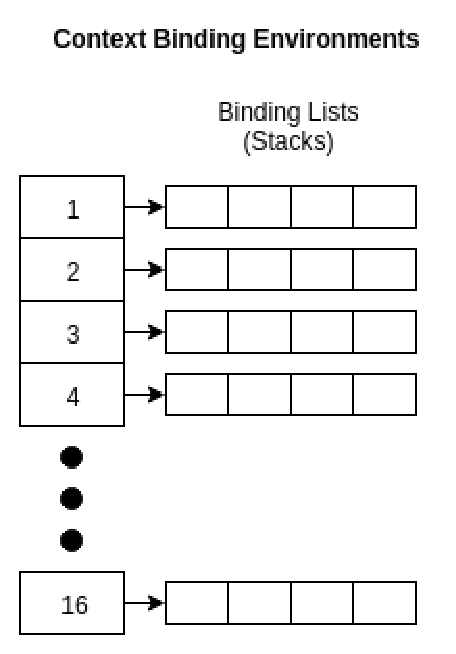
\includegraphics[scale=0.75,natwidth=203,natheight=298]{context}
\caption{The binding environment inside a context used to store the length and offset of fields, or the offset of headers. On the left, indexes one through sixteen represent the fields that can be extracted. Each field maintains a binding stack. Each element in the binding stack is a binding which stores the offset and length where an instance of that field can be found. }
\label{fg:ContextEnv}
\end{figure}

Since any given packet can contain one or more of any field or header with the same name, a binding environment maintains a stack for every field and header. These stacks are called \textit{binding stacks}. By extension, this means an environment is actually a mapping of field names to binding stacks. When the value of a field is needed, the topmost binding on the binding stack shall be used to recover the value of that field.

The implementation of a binding environment in Flowpath is a fixed-sized array where each element in the array is a fixed-sized binding stack. Each valid index in the array represents a unique field or header name extracted by the Steve application. The compiler is responsible for associating all unique field names to unique integer indexes. The same is done for all unique headers. This provides constant time lookup of field bindings without the overhead of hashing complex names.

Figure \ref{fg:ContextEnvWorking} demonstrates how data is stored in the context as it is being decoded. The example is a packet which contains an encapsulated IPv4 header commonly used in IP tunneling. In the ethernet decoding stage which extract the \texttt{src}, \texttt{dst}, and \texttt{type} field are extracted and stored in the context. Next we determine that IPv4 follows based on the \texttt{type} field. We extract IPv4 \texttt{dst} and \texttt{protocol}. The \texttt{protocol} field tells us we have another IPv4 header after the current one. We move to decode that and once again we extract IPv4 \texttt{dst} and \texttt{protocol}. Note how the new values of IPv4 are pushed on top of the binding stack. Any further usage of those fields will use the latest values extracted for those fields. Keep in mind that this means any usage of the first set of IPv4 \texttt{dst} and \texttt{protocol} must occur before the decoding of the second IPv4 header.\

\begin{figure}
TODO: Make an image for this.
\caption{A context environment in action during runtime.}
\label{fg:ContextEnvWorking}
\end{figure}

The \textbf{action set} is the other major data structure contained within the context. Actions are written to the action set for \textit{deferred execution} through the course of a pipeline. These actions are executed once the pipeline is complete, during the egress processing phase.

\section{Decoding Stage} \label{decoder_desc}

When a packet is received on its ingress port, it is a chunk of raw, uninterpreted data. Before a packet can be processed and routed, its headers and fields must be decoded and extracted so that meaningful decisions can be made about based on those values. The decoding stage is responsible for this.

Steve allows for programmers to specify \textit{how} and \textit{which} fields are extracted from headers. In other paradigms, the \textit{entire} packet is decoded from start to finish; all headers and all fields are extracted, then all fields are saved. This is what is considered a \textbf{full decode}. After this full decode, the decision making process on the packet begins using those saved fields. However, this method is inherently inefficient. Only certain fields and headers within a packet are ever really needed. To compound this, different devices may care about different subsets of fields within a given packet. Decoding all headers and fields from a packet is inherently wasteful.

Full decodes waste valuable processing time. Efficiency is important when dealing with networking equipment which has to processes between 10Gbps to 40Gbps. This inherent inefficiency is why Steve proposes the idea of a \textit{partial decode}. Unlike similar SDN-focused programming languages, Steve is designed to allow programmers to specify the extraction of only specific fields rather than an entire header. Though the specification may be verbose in some cases, it makes programmers think very carefully about which fields they need and which fields they do not. 

Additionally, Steve proposes that not all headers need to be decoded. For example, if a networking application only needs to forward using MAC addresses, there is no reason to waste time extracting fields from IPv4 or IPv6 headers, and so on.

That being said, Steve also supports the full decode. It may be desirable to some programmers to do this in certain scenarios, thus the language does not favor one paradigm over another.

\section{Table Stage} \label{table_desc}

Table stages handle matching against extracted fields, i.e. classification, and perform a sequence of desired actions on like-classified packets. This is done through a mechanism known as a flow table defined by the OpenFlow standard \cite{openflow_spec}.

A \textbf{flow table} is composed of a set of \textbf{flow entries}. A flow entry is composed of \textbf{match fields}, a \textbf{priority}, a set of \textbf{actions}, and miscellaneous additional data. Each table specifies a set of key fields that together make up a \textbf{key} for that table. For each key field, each flow entry has a corresponding value, known as a \textbf{match field}, such that every flow entry in the table is uniquely identified by its match fields and its \textbf{priority}.

When a packet reaches a table matching stage, the fields comprising the table's key are extracted from the context. Lookup into the table retrieves all flow entries whose match fields can correctly match the field values from the packet. The flow entry whose priority is highest is selected. The \textbf{actions} of the flow entry are executed on the packet.

If no such flow entry matches against the packet's field values, the \textbf{miss case} flow entry is applied to the packet instead. Flow entries can be user defined. By default, a miss in a table results in the packet being dropped. Miss cases always have the lowest possible priority amongst flow entries and each match field can be considered a wildcard.

The mechanic of table matching is not distinctly different from those of relational or SQL tables. In fact, Frenetic, another packet processing language, uses SQL-inspired syntax to classify flows \cite{frenetic_paper1}. If we make this comparison, a flow table is analogous to a SQL table, the concept of a key is the same for both, and a flow entry is analogous to a tuple in a SQL table. Each packet and its fields constitute the actual "query" into the table.

\section{Pipeline Composition} \label{pipeline_comp_desc}

Kinds of processing stages can be interleaved together in any order within the pipeline. This means that Steve is capable of supporting different packet processing paradigms found in other research such as POF and P4. With the Steve pipeline specification language a user can specify that a pipeline does:

\begin{enumerate}
\item \textbf{A full decode of the packet followed by a sequence of tables.} Packets coming to the pipeline have all necessary headers and fields are decoded and saved in the runtime context first. The packet is then dispatched to the first table in the pipeline. From there, matched flows within the tables dictate which table the packet is sent to next or which port the packet is forwarded to.
\item \textbf{A chain of partial decodes and table lookups.} Packets coming to the pipeline get partially decoded and dispatched to a table. The flow within that table could carry the packet to another table, another decoder, or forward it out of the network. The pipeline in this case in a chain of alternating sequences of decoding stages and table matching stages.
\item \textbf{Only decodes.} In some special cases, it may not even be necessary to go to a table matching stage. It may be possible to make a decision about the packet’s ultimate destination immediately upon evaluating a certain field within the packet using a simple conditional statement (if-statement, if-else statement, etc). Therefore, decoding stages also support the range of actions supported by flow entries, which can include outputting packets to a port or dropping it.
\end{enumerate}

Upon entering the pipeline, a packet must first go through at least one decoding stage before moving to the next processing stage. From there, the packet flows from one stage of the pipeline to the next. With each stage, certain conditions are evaluated which will determine where the packet must flow next. Finally, the packet will exit the pipeline either through a port(s) or by being dropped and discarded.

\chapter{Flowpath} \label{ch:flowpath}

Flowpath is a programmable, protocol oblivious, software data plane which is part of the Freeflow project \cite{freeflow_software}. Flowpath exposes an API to allow other programs to configure and program it through its runtime environment. Flowpath is designed to load dynamic link libraries known as \textit{Flowpath pipeline applications}. 

Flowpath pipeline applications expose their own API, which must conform to a certain specification to be \textit{Flowpath loadable}. 
They will use the Flowpath API to provide packet decoder's, configure the data plane's flow tables and flow entries, provide event handlers for exceptional events, and control the logic behind the packet processing pipeline.

For now, Steve is specifically tailored toward compiling Flowpath pipeline applications. This chapter will focus on Flowpath, its interactions with Steve, and how Steve applications leverage the Flowpath API to create packet processing pipelines.

\section{Flowpath}

The Flowpath runtime environment abstracts the low-level hardware and software resources. This includes port management, packet reading, memory management, flow table allocation, and table matching algorithms. Flowpath does \textit{not}, however, specify its own packet processing pipeline. Packet decoders, flow table configuration details, flow entry definitions, and exceptional event handling is left up to the pipeline application which Flowpath loads.

Flowpath also supports multitenancy, that is, it provides the ability to construct multiple instances of software data planes on a single machine.

\section{Runtime Configuration} \label{config_guide}

Steve applications are shared object libraries (.so files). They are not, by themselves, executable. They must be loaded by an instance of the Flowpath runtime. In order to do this, a C++ driver must be written for the Flowpath runtime which will load the Steve application. Flowpath will expect that Steve supports three interface functions. These functions get executed in a specific order once the Steve application is loaded.

\begin{enumerate}
\item \textit{Configuration}. The first thing Flowpath will do is call the Steve application's configuration function. This function allows Steve to make requests for tables and initial flow entries. The Steve application will ask for a table with a certain ID number, size, and key width. Flowpath will allocate such a table and return a handle to the table back to the Steve application. Once the handle is received, the Steve application will request that all initial flow entries are inserted into the table. Next, all ports declared with an initial port initializer are requested. If they exist, then their identifiers are return, otherwise the identifier to the invalid port (i.e. zero) is returned.

\item \textit{Port Changed Notifications}. If a port has changed, then a notification is sent to the Steve application about that change. A port change notification may state whether a port has gone up or down. If a port has gone up, then an uninitialized prot declared by the Steve application is set to that port. If a port has gone down, then any declared port with that value is set to the invalid port (i.e. zero).

\item \textit{Process}. Flowpath will begin sending contexts to the Steve application for pipeline processing through this interface.
\end{enumerate}

\section{Egress Processing} \label{egress_process}

Egress processing occurs right before a packet is forwarded. Egress processing begins when a pipeline processing stage (decoder, event, or table) has finished, but has not sent the context to another stage. At this time, actions written to the context's action set are executed. These actions may have special semantics when executed at this time (see \ref{guide:write}). Each action is executed in the order with which it was written. Once the action set is finished executing, the forwarding decision is made.

The context's output port field indicates which port to forward the original packet on. If the output port field is not set, the packet will be dropped and deleted from memory. Once the packet has been forwarded, the context memory is deleted. 
\chapter{The Steve Language} \label{ch:tutorial}

% It might be worthwhile to divide this into three major sections:
%
% 1. General purpose computing
% 2. Packet specification
% 3. Pipeline specification
%    - decoders
%    - flow tables

The Steve Programming Language provides features for
defining and connecting the pipeline processing stages and event handlers. Together, these components comprise a network application.

%After the first example, this chapter will delve into all the individual pieces of a Steve program with additional details and use cases.
This chapter will describe all of the language features for Steve in greater detail with use cases.
Specifically, this chapter will discuss how headers are represented (Section \ref{tut:layout}), how to
write decoders (Section \ref{tut:decoder}), how to write flow tables (Section \ref{tut:table}), how to apply actions to packets (Section \ref{tut:action}), and how to write event handlers (Section \ref{tut:event}).

Semantics and limitations of Steve will be mentioned throughout this chapter, 
but not in complete detail. For the complete semantic description of
Steve, including grammar, typing rules, and other restrictions, see the Reference Guide in Appendix \ref{ch:users_guide}.

\section{General Purpose Language Features} \label{tut:gen_purp}

Steve supports language features that can be considered
\textit{general purpose}. They are common to most programming
languages and are not explicitly for packet processing, though they may prove
useful.

%\subsection{Literals} \label{tut:literal}
%
%Steve supports decimal, binary, and hexadecimal integer literals. Steve does not
%currently support things like IP address literals or MAC address literals.
%
%Hexadecimal literals all start with the prefix \texttt{0x} followed by any
%number of digits between \texttt{0} and \texttt{9}. Binary literals all start with the prefix \texttt{0b} followed by any number of
%\texttt{0}'s and \texttt{1}'s.
%These integer literals can be written as follows.
%
%\begin{codepage}
%\begin{lstlisting}
%17 // Decimal literal
%0x11 // Hexadecimal 17
%0x00010001 // Binary 17
%\end{lstlisting}
%\end{codepage}
% 
%The underscore (\texttt{\_}) can optionally be used as a digit separator (like 
%Java) for hexadecimal and binary literals with no impact on the value of that 
%literal.
%This is purely for organization and readability.
%
%\begin{codepage}
%\begin{lstlisting}
%0b10101010
%0b1010_1010
%
%0x0800
%0x08_00
%\end{lstlisting}
%\end{codepage}
%
%Steve also supports character and string literals which are useful for
%logging through C library functions (described in Section \ref{tut:foreign}).

\subsection{Variables} \label{tut:variable}

Steve allows for the allocation of both local and global variables. 
A variable named \texttt{x} which holds an integer \texttt{10} is written
as follows. 

\begin{codepage}
\begin{lstlisting}
var x : int = 10;
x = 9; // Assign a new value.
\end{lstlisting}
\end{codepage}

\subsection{Conditional and Loop Statements} \label{tut:condition}

Steve supports two conditional statements for decision making: the \texttt{if} statement and the \texttt{match} statement. 
The \texttt{if} statement is the same as C.

A \texttt{match} statement allows for a decision to be made given a number of 
possible case values. 
This is similar to a C-like switch statement, with the only
major difference being that there is no \textit{fall-through} behavior. In other
words, after the execution of a \texttt{case} statement, control jumps out of the 
\texttt{match} statement rather than moving to the next case (i.e. an implied 
\texttt{break}). 
The condition and labels must be integers just like in C. 
A \texttt{match} statement can be written as follows.

\begin{codepage}
\begin{lstlisting}
match (x) {
  case 0: x = x + 1;
  // Multiple statements following the label must be
  // enclosed in a block.
  case 1: {
    x = x + 2;
    y = y * x;
  }
  // The default case statement.
  miss: x = 0;
}
\end{lstlisting}
\end{codepage}

Steve also supports the \texttt{while} loop which is the same as C-like languages. 
It also supports the \texttt{break} and \texttt{continue} statements for limited
branching abilities inside a loop. 

\subsection{Functions} \label{tut:function}

Steve supports writing simple functions, though the syntax is a little different
from C-like languages.
A function named \texttt{sum} which takes two
integers, \texttt{a} and \texttt{b}, and returned their sum is written as follows.
The return type follows the \texttt{->} in Steve functions.

\begin{codepage}
\begin{lstlisting}
def sum(a : int, b : int) -> int {
  return a + b;
}

sum(1, 2);
\end{lstlisting}
\end{codepage}

\subsection{Foreign Functions} \label{tut:foreign}

By default, all Steve compiled applications are linked against the C runtime
library. Steve applications may also be linked against other libraries.
Steve programmers may call functions in linked libraries by first declaring
them in the Steve application using a \emph{foreign function} with the same
function signature.

\begin{codepage}
\begin{lstlisting}
foreign def puts(input : char[]) -> int;

puts("Hello, World.");
\end{lstlisting}
\end{codepage}

Here, this foreign function links to the C standard \texttt{puts} function
for text output. It may be called like any other function.

\section{Layouts} \label{tut:layout}

A \textit{layout} is used to describe 
the \textit{structure} of a packet header.
More specifically, they describe \textit{what} fields are present, their
\textit{lengths}, the \textit{order} in which they appear, and their
\textit{relative offset} from the beginning of the header. 
Decoders use layout information to reason about extracting fields.

%A layout and a header are two different concepts.
%It is important to make this distinction clear. A layout is like a blueprint for
%a header. It gives us information; it \textit{describes} that header. The header
%is an actual sequence of bits, a portion of the packet, which is taken off of the
%network. The header \textit{exists} whereas a layout helps the Steve application
%\textit{understand} it.

A \emph{layout declaration} (see \ref{guide:layout}) is used to write a layout.
The simplest example to begin with is the Ethernet frame header \cite{eth_std}.
The corresponding layout would look like the following.  

\begin{codepage}
\begin{lstlisting}
layout ethernet {
	dst  : uint(48); // 48 bits.
	src  : uint(48); // 48 bits.
	type : uint(16); // 16 bits.
}
\end{lstlisting}
\end{codepage}

Every layout has a name (\texttt{ethernet}) and a sequence of field declarations
which describe the fields contained within the header.
This layout has three such field declarations (\texttt{dst}, \texttt{src},
and \texttt{type}).
Each field declaration has a name and a type that describes valid operations and
value ranges for that field.
To reduce errors related to working with byte buffers, Steve allows header fields to
be represented as fixed-precision, signed or unsigned, integer types.
The precision denotes the length of the field in bits.
Here, \texttt{dst} and \texttt{src} fields are 48 bits long and \texttt{type} is
16 bits long.

The \textit{relative offset} of each field is the number of bits it is away
from the beginning of the header. The first field will always have a relative
offset of 0 bits. The relative offset of each subsequent field is equal to the
sum of the lengths of all fields preceding it. Here, \texttt{dst} has a relative
offset of 0 bits, \texttt{src} has one of 48 bits (6 bytes), and \texttt{type} has one of
96 bits (12 bytes).

The field declarations must appear in the order with which they would normally appear
in an Ethernet header. Field ordering should always be
preserved when declaring layouts. If the ordering is incorrect, decoders will
assume a sequence of bits is a certain field when it truly is not. 

Not all header structures are as simple as the Ethernet header. Sometimes one
must deal with structures encapsulated inside a header. Steve supports composition of layouts to describe such header structures.
The following presents an OpenFlow protocol message which contains such a case \cite{openflow_spec}.

\begin{codepage}
\begin{lstlisting}
layout ofp_instr_stat_trigger {
	type : uint(16); 
	len : uint(16); 
	flags : uint(32); 
	threshold : ofp_stats;
};

layout ofp_stats {
	reserved : uint(16); 
	length : uint(16); 
	oxs_field : uint(8);
	padding : uint(32);
};
\end{lstlisting}
\end{codepage}

In this example, two layouts are presented: \texttt{ofp\_instr\_stat\_trigger} and \texttt{ofp\_stats}. 
To express the \texttt{ofp\_stats} structure within the OpenFlow message, a field named \texttt{threshold} is added to
\texttt{ofp\_instr\_stat\_trigger} and its type is given as the name of another layout (\texttt{ofp\_stats}). The length of the \texttt{threshold} field would be the sum of the lengths
its fields, in this case, 72 bits (9 bytes).

With the way
layouts are described and written, it is easy to draw the comparison between 
layouts and
class types (or record types). \textit{Layouts are not 
classes.} Layouts are much stricter.

First, \textit{the types of fields are restricted}. Fields may only
have two types: integer (see \ref{guide:integer_type}) and layout
(see \ref{guide:layout_type}). There may be varying kinds of integer (e.g.
precisions, signed, unsigned, etc.), but the precision of each integer must also
be \textit{byte-aligned}, that is, a multiple of 8.

Second, the most important distinction is that \textit{objects of layout type
can never be created}. Layouts may not appear as the type of parameters, nor may
they appear as return types. All of the following are considered ill-formed.

\begin{codepage}
\begin{lstlisting}
layout L1 { f1 : uint; f2 : uint(16); }
var x : L1 = 0; // Error.
def foo(y : L1) -> L1 { ... } // Error.
\end{lstlisting}
\end{codepage}

Layouts are distinct from the headers that they describe.
The sole purpose of layouts is to allow decoders to reason about the logical 
structure of a header in memory.
The memory for packets and their headers exist independent of a running Steve 
application.
To create an object of layout type would imply the need to create new headers,
which is not currently supported by Steve.

%Additionally, there are a number
%of concerns related to constructing objects of layout type, thus such behavior
%is not allowed. For further details on layout limitations, refer to Section
%\ref{guide:no_dst} in the Reference Guide.

Another important thing to note is that Steve does not currently support dynamically
sized types (DST). A DST is a type whose size is predicated upon some value
known only during runtime. These DST's are used to represent fields whose
lengths are dynamic. Some examples of dynamic length fields are the
\texttt{options} fields in IPv4, IPv6 extended, and TCP headers \cite{ipv4_std, ipv6_std,
tcp_std}.

DST's are a language feature that will eventually be added, but are outside the
current implementation. Because of this, fields whose lengths are dynamic cannot
currently be declared, extracted, nor used. The existence and eventual support
of DST's is one of the reasons why objects of layout type cannot be created.
This is further discussed in Section \ref{guide:no_dst}.

The following example presents a case where some of these limitations become relevant -- the IPv4 layout.

\begin{codepage}
\begin{lstlisting}
layout ipv4 {
  version_ihl : uint(8); // Non-byte aligned fields are merged
  dscp_ecn    : uint(8); // This is merged, too.
  len         : uint(16);
  id          : uint(16);
  fragment    : uint(16); // Fragment flags and offset merged.
  ttl         : uint(8);
  protocol    : uint(8);
  checksum    : uint(16);
  src         : uint(32);
  dst         : uint(32);
  // Options field omitted because it is a DST.
}
\end{lstlisting}
\end{codepage}

In this example, \texttt{version} (a 4 bit field) has to be
merged with \texttt{ihl} (internet header length) (also a 4 bit field) to
achieve byte alignment. The same is true for \texttt{dscp} and \texttt{ecn}. The
\texttt{fragment} field, typically composed of three 1 bit flags and a 13 bit
fragment offset field, is merged into a single 16 bit field. 
Bitwise-AND and bit shifting is needed to recover the needed bits.
Examples will come up later when an IPv4 decoder is discussed in
Section \ref{tut:decoder_access}.

\section{Decoders} \label{tut:decoder}

Decoders are special purpose functions
used to extract fields from a single header. 
They implicitly take context data structures as arguments and 
operate on them.
A decoder conforms to a layout specification.
Layout information allows the decoder to determine where fields
are located in a header and how long they are.


%\begin{itemize}
%\item Which header is being decoded?
%
%\item What fields from the header are needed and why?
%
%\item How will these fields be used? Will they be used in arithmetic or 
%
%\item \textit{Actions} (described later in Section \ref{tut:action}) are used to manipulate packet fields, forward packets,
%and add/remove flow entries from tables. What actions must be be taken on the packet?
%
%\item Where must the packet be sent next? Must it be further decoded or can it be sent to table matching for decision making?
%\end{itemize}

\subsection{The Basic Decoder Form} \label{tut:basic_decoder}

A decoder is written using a \textit{decoder declaration} (see \ref{guide:decoder}).
The most common decoder written is likely the Ethernet decoder. The following
is the basic form of an Ethernet decoder.

\begin{codepage}
\begin{lstlisting}
decoder start eth_d(ethernet) { ... }
\end{lstlisting}
\end{codepage}

A decoder declaration has four important parts: 
1) a name (\texttt{eth\_d}), 
2) a \textit{layout rule} (\texttt{ethernet}),
3) a body, and
4) the optional \texttt{start} keyword.

The decoding process conforms to the layout rule and uses it to reason
about the location and lengths of fields within the header it is decoding.
Decoder operations are placed in the body delimited by $\lbrace\rbrace$.
The \texttt{start} keyword identifies this decoder as the \emph{starting
decoder}. 

A starting decoder is the root of the pipeline.
By extension there can only be one starting decoder.
Every packet must be processed by the starting decoder first.
Since Ethernet is the most common Layer 2 framing protocol, it will
likely be the root of almost all pipelines.

\subsection{Extractions} \label{tut:decoder_extract}

An \textit{extract declaration} (see \ref{guide:extract}) in the decoder's body
instructs it to extract the given field. Extracted fields, or \emph{extractions},
for short, may then be used by the program as a variable.
The following example expands the body of the \texttt{eth\_d} decoder 
with extract declarations.

\begin{codepage}
\begin{lstlisting}
decoder start eth_d(ethernet) {
	extract ethernet.dst;
	extract ethernet.type;
	// ...
}
\end{lstlisting}
\end{codepage}

Each extract declaration gives a \emph{field name} (see \ref{guide:field_name}) 
which tells the decoder which field is being extracted. 
In this example, there are
two such extract declarations which instruct the decoder to extract
the fields \texttt{ethernet.dst} and \texttt{ethernet.type}.
The compiler generates \textit{(offset, length)} pairs 
denoting the relative offset and length of the field within the decoder's view using the given field names and layout rule. 

Only field names which refer to fields in the layout rule may be used. It obviously make no sense to extract a field not in the header. 
For example, it would not be possible to extract \texttt{ipv4.protocol} in the \texttt{eth\_d} decoder. 

\subsection{Accessing Extracted Fields} \label{tut:decoder_access}

Once a field has been extracted, getting its value is similar to using
it as variable.
To get the value of an extraction
the \textit{field access expression} (see \ref{guide:field_access_expr}) is used.
A field access expression is a field name being used where
an expression is expected. This is similar to using a variable name
in an expression to represent the value of the variable.

A typical operation on an Ethernet header is determining which protocol
it encapsulates, i.e. the header which comes next. This is indicated
by the value stored in \texttt{ethernet.type}.
The following example demonstrates how the value of the \texttt{ethernet.type} 
extraction might be used.

\begin{codepage}
\begin{lstlisting}
decoder start eth_d(ethernet) {
  extract ethernet.dst;
  extract ethernet.type;
  if (ethernet.type >= 0x600) {
    // The type determines what header comes next...
  }
  else if (ethernet.type <= 0x05dc) {
    // The type is the length of the entire packet...
  }
}
\end{lstlisting}
\end{codepage}


The IEEE Ethernet standard says that \texttt{ethernet.type} fields greater than 
or equal to \texttt{0x600} indicate the next header's protocol \cite{eth_std}. 
Any \texttt{type} fields less than \texttt{0x05dc} indicate the Ethernet frame's 
length. 
Here, field access is used to compare \texttt{ethernet.type} to 
hexadecimal literals in an \texttt{if-else} statement to determine the meaning of 
that field.

Extraction values can also be used in arithmetic operations, comparison 
operations, bitwise operations, function calls,
and can be stored and assigned to variables. The following example presents
a trivial IPv4 decoder demonstrating some of these basic operations.

\begin{codepage}
\begin{lstlisting}
decoder ipv4_d(ipv4) {
  extract ipv4.version_ihl; // Use this to get header length.
  extract ipv4.dscp_ecn;
  extract ipv4.len;
  extract ipv4.id;
  extract ipv4.fragment;
  extract ipv4.ttl;
  extract ipv4.protocol;
  extract ipv4.checksum;
  extract ipv4.src;
  extract ipv4.dst;
  
  var pktlen : uint = ipv4.len; // Variable assignment
  var ihl : uint(8) = ipv4.version_ihl & 0x0f; // Bitwise AND
  var version : uint(8) = ipv4.version_ihl >> 4; // Shift
  // ...
}
\end{lstlisting}
\end{codepage}

This example presents a solution for recovering non-byte aligned
fields. A bitwise-AND (see \ref{guide:bitwise_expr}) is used on \texttt{ipv4.version\_ihl}
with \texttt{0x0f} to recover the \texttt{ihl} field. The 
\texttt{ipv4.version\_ihl} is left-shift by 4 bits to get the \texttt{version} field.

Extractions can be passed to functions as well. A convenient use case is 
calculating the checksum for the IPv4 header. 
The following example extends the IPv4 decoder with a few more operations.

\begin{codepage}
\begin{lstlisting}
decoder ipv4_d(ipv4) {
  // ...
  // Calculate a checksum by calling a function.
  var checksum : uint(16) =
      ipv4_checksum(ipv4.version_ihl, ipv4.dscp_ecn, ipv4.len, 
                    ipv4.id, ipv4.fragment, ipv4.ttl, 
                    ipv4.protocol, ipv4.src, ipv4.dst);
  // Check the checksum against the header's checksum.
  if (checksum != ipv4.checksum)
	  drop;
  // Drop time-to-live expired packets.
  if (ipv4.ttl == 0)
    drop;
  set ipv4.ttl = ipv4.ttl - 1; // Decrement time-to-live
  // The ttl has changed. A new checksum must be calculated.
  set ipv4.checksum =
    ipv4_checksum(ipv4.version_ihl, ipv4.dscp_ecn, ipv4.len, 
                  ipv4.id, ipv4.fragment, ipv4.ttl, 
                  ipv4.protocol, ipv4.src, ipv4.dst);
}
\end{lstlisting}
\end{codepage}

Fields from the IPv4 header are passed to a function named 
\texttt{ipv4\_checksum} (whose definition has been elided for brevity). The 
resulting checksum is compared against the current checksum using an \texttt{if} 
statement. If they do not compare equal, then the packet is dropped using the 
\texttt{drop} action.

Decrementing the time-to-live (\texttt{ipv4.ttl}) is also a common operation. 
First the time-to-live is checked to see if it is \texttt{0}. If it is, then the 
packet's lifetime has expired and it will be dropped. If the packet is still 
valid, the field is decremented using simple subtraction and the 
\texttt{set} action. Because a field has been changed in the IPv4 
header, the checksum must be recalculated and set with the new checksum.

Field access expressions do have a number of limitations. The following example
demonstrates some of them.

\begin{codepage}
\begin{lstlisting}
decoder start eth_d(ethernet) {
  // Error: Cannot use eth.type before its extracted.
  if (ethernet.type >= 0x600) { }
  extract ethernet.type;
  // Error: Cannot assign to a field this way.
  ethernet.type = 0x800;
  // OK: A set action must be used instead.
  set ethernet.type = 0x800;
}

decoder ipv4_decode(ipv4) {
  // Error: This decoder does not decode ethernet.
  extract ethernet.type;
  // Error: ethernet.type was not extracted by this decoder.
  if (ethernet.type == 0x800) { }
}
\end{lstlisting}
\end{codepage}

A field access expression can only be used \textit{after} an extract declaration
is made for that field since it is impossible to recover the value of a
field which has not been extracted. By extensions, they cannot be used inside a
decoder that has not extracted that field even if a prior decoder extracted that field. A decoder focuses on exactly one
header and has no knowledge of previous headers or extractions.
Field access expressions are not the same as variables and may not be assigned to like one. To modify the
value of a field, a \texttt{set} action must be used instead.

\subsection{Rebinding Extracted Fields}

The context binding environment
allows fields to be rebound with different names. This essentially
allows the a field to be referred to using a different name.
When extracting multiple fields of the same name, this allows the
programmer to disambiguate them. 

More commonly it is used to rename fields so that they may be reinterpreted as other fields. For example, assume that an Ethernet
frame has a VLAN tag. The \texttt{ethertype} field of the VLAN tag is what 
actually informs the switch what Layer 3 protocol is encapsulated
by Ethernet. 
A rebind declaration (\ref{guide:rebind}) is used to alias a field with a new name.
So for example:

\begin{codepage}
\begin{lstlisting}
layout vlan {
	tci : uint(16);
	ethertype : uint(16);
}

decoder start eth_d(ethernet) {
	extract ethernet.type;
	match(ethernet.type) {
		case 0x8100: decode vlan_d;
	}
}

decoder start vlan_d(vlan) {
	extract vlan.ethertype as ethernet.type; // Rebind
	goto ethtable;
}
\end{lstlisting}
\end{codepage}

In \texttt{vlan\_d}, the \texttt{extract vlan.ethertype as ethernet.type} allows the extraction of \texttt{vlan.ethertype} to be referred to as
\texttt{ethernet.type} in future stages. The \texttt{vlan.ethertype}
is the \emph{original} field and \texttt{ethernet.type} is the \emph{alias} field.
Consider the following table:

\begin{codepage}
\begin{lstlisting}
exact_table ethtable(ethernet.type) {
	{ 0x8100 } -> { ... }
	{ 0x86dd } -> { ... }
}
\end{lstlisting}
\end{codepage}

Assume that \texttt{vlan.ethertype} has a value of \texttt{0x86dd}.
When \texttt{vlan\_d} sends the packet to \texttt{ethtable}, it will
match the flow entry whose match field is \texttt{0x86dd}. Because of
the rebind \texttt{ethernet.type} refers to the extracted \texttt{vlan.ethertype}.


\subsection{Stage Transition} \label{tut:decoder_next}

Once the current stage has finished its work, the programmer may decide
to send the packet to another pipeline stage.
Section \ref{pipeline_comp_desc} describes that decoding and
table matching stages can be chained together in a number of flexible ways.
Any stage may move a packet to a new decoder or a new table.

To move to another decoding stage, the \texttt{decode} action (see \ref{tut:decode_action})
is used. The following example bridges the Ethernet and IPv4 decoders
declared in earlier examples. Extract declarations are elided for
brevity.

\begin{codepage}
\begin{lstlisting}
decoder start eth_d(ethernet) {
	// ...
	if (ethernet.type >= 0x600)
	    match (ethernet.type) {
	      case 0x800: decode ipv4_d;
	    }
}

decoder ipv4_d(ipv4) { ... }
\end{lstlisting}
\end{codepage}

The \texttt{match} statement is used to check if \texttt{ethernet.type} is equal to
\texttt{0x800}. If it is, then it confirms the next header is IPv4 and the \texttt{decode} action moves the packet to the IPv4 decoder.

To transition to a table matching stage, a \texttt{goto} action (see \ref{tut:goto_action}) (not
to be confused with a C-like \texttt{goto}) is used.

\begin{codepage}
\begin{lstlisting}
decoder ipv4_d(ipv4) {
  // ...
  var ihl : uint(8) = (ipv4.version_ihl & 0x0f) * 4;
  // Advance specifier shifts the view by N bytes.
  goto tcp_filter advance ihl; // tcp_filter names a table.
}
\end{lstlisting}
\end{codepage}

In this example, the \texttt{goto} action sends the packet to a hypothetical table
named \texttt{tcp\_filter}. Details about writing tables follows in Section \ref{tut:table}. 
The most important thing to notice from this example is the
\texttt{advance} specifier.

Section \ref{tut:extract_how} explains that a decoder shifts the
\textit{view} of a packet before moving to the next stage. That shift is by the
length of the header. IPv4 headers are dynamic in length. Even though Steve does not
currently support extracting dynamic length fields, one must still account for
them. To correctly do this, the \texttt{advance} specifier is applied to
explicitly shift the view by the given number of \textit{bytes}. 
Here, the \texttt{ihl} calculation determines the number of bytes in the header.
The assumption is made that all headers are byte-aligned, therefore advancing by
a number of bytes (rather than bits) is appropriate. 

The \texttt{advance} specifier may appear on both \texttt{goto} and \texttt{decode} actions. However, it may only appear in a decoder, as decoders are the only
stage concerned with views.

A stage is \textit{complete} once it executes a \texttt{decode} or \texttt{goto} action, or
finishes executing without either action being executed. 
These two actions are similar in semantics to a function return
in that the stage will not execute anything after them.
If no stage transition happens at all,
the packet exits the pipeline and enters egress processing.

Actions appended to the context's action list are executed before a forwarding decision is made.
The original packet is forwarded based on the egress port field stored
within the packet context. This field is set when executing an
output action that has been written to the context's action list
(see \ref{tut:write_action}) for an example). If this field was not set,
then the packet is implicitly dropped.

\section{Tables} \label{tut:table}

The next stage is the table matching stage which uses the flow table mechanism described in Section \ref{table_desc} to direct network flows. Flow tables are decision tables that are built into the language.

\subsection{The Basic Table} \label{tut:basic_table}

The following example presents the basic form of a table which
groups TCP packets by destination port. The definition of the TCP
layout has been elided here, but may be found in Section \ref{tut:firewall}.

\begin{codepage}
\begin{lstlisting}
exact_table tcp_filter(tcp.dst) {
	// Flow entries...
}
\end{lstlisting}
\end{codepage}

Each flow table is comprised of three parts: 
1) a name (\texttt{tcp\_filter}), 
2) a \textit{key}, and
3) a set of \textit{flow entries}. 
Additionally, there may be three kinds of flow tables: 
\textit{exact}, \textit{prefix}, and \textit{wildcard}. 
This is an exact match table (Steve currently only supports exact
match tables).

A table's \textit{key} provides a comma-separated list of field names, known as
\textit{key fields}, which indicate which protocol fields a table matches on.
They are the equivalent of decision attributes. 
The \texttt{tcp\_filter} table matches on a single field (\texttt{tcp.dst}).

It is important to note that a \texttt{goto} action may only dispatch
a packet to a table if the key fields have been extracted in prior decoders. This ensures that the key fields actually exist before matching begins. If they have not been extracted, the program is ill-formed. How the compiler checks this is explained in Section \ref{guide:requirements}.

Flow entries define the criteria for a network flow, and
what actions are taken on packets belonging to those flows.
They are the rules of a decision table.
To write a flow entry, a \textit{flow entry declaration}
(see \ref{guide:tables}) is used.
The following example presents three flow entries:
two regular ones followed by a special one known as the \emph{miss case}.

\begin{codepage}
\begin{lstlisting}
exact_table tcp_filter(tcp.dst) {
	{ 80 } -> { goto forward; }
	{ 443 } -> { goto forward; }
	miss -> { drop; }
}
\end{lstlisting}
\end{codepage}

A flow entry declaration has two parts: 1) \textit{match
fields} and 2) an \textit{action sequence} (also called the body of the entry). 
Match fields appear as a comma-separated list of expressions 
in the brace-enclosed block (\{\}) before the \texttt{->}. 
The first two flow entries have a single match field each --
\texttt{80} and \texttt{443}, respectively.

Match fields are values which correspond to the table's key fields. 
When a packet is matched against a table,
the table compares the packet's fields with the match fields of each flow entry.
A packet \textit{matches} a flow entry if each field (which is part of the
table's key) in the packet matches each corresponding match field in the flow 
entry. 

The action sequence is given in the brace-enclosed block (\{\}) after the \texttt{->}. When a packet matches a flow entry, actions in this
sequence are executed.
In this example, if a packet's TCP destination port field is equal to \texttt{80},
then it will match the first flow entry and it will be sent to another flow table
named \texttt{forward}. The same is true for packets whose TCP destination
port field is equal to \texttt{443}.

The third flow entry is a special entry known as the \textit{miss case}. The miss 
case uses the keyword \texttt{miss} rather than providing match fields. If no 
other flow entry in a table can match a packet, the miss case is used. A table 
may only have one miss case. If one is not given, an implicit one exists which 
is the equivalent to the second flow entry in the example. That is, by default 
miss cases drop a packet.

Flow entries declared within a flow table body are known
as \textit{initial flow entries}. 
They get installed when a Steve application is loaded by the runtime.
Flow entries may also be added to a flow table after it has begun processing packets. 
An example of adding and removing flow entries can be found in Section \ref{tut:insert_flow_action} and \ref{tut:remove_flow_action}, respectively.

\subsection{A More Complex Table} \label{tut:complex_table}

The \texttt{tcp\_filter} table from Section \ref{tut:basic_table} is only the most basic of flow tables. 
Flow tables can have more complicated use cases.
Not all flow tables will match on a single field. In fact, most flow tables will
match on many fields. The following table declaration demonstrates this.

\begin{codepage}
\begin{lstlisting}
exact_table ip_proto(ipv4.fragment, ipv4.protocol) {
  { 0x0, 0x11 } -> { decode udp_d; }
  // And so on...
}
\end{lstlisting}
\end{codepage}

This table classifies packets into flows based on their fragment value
and the IP encapsulated transport layer protocol. This flow entry
groups non-fragmented, UDP packets.

Flow entries may also have \textit{properties}. Properties are additional
information stored alongside flow entries. 
Steve currently supports two properties: timeout and egress.
The following example extends the previous \texttt{ip\_proto} table with a new flow entry using the timeout property.

\begin{codepage}
\begin{lstlisting}
exact_table ip_proto(ipv4.fragment, ipv4.protocol) {
  { 0x0, 0x06 } ->
  [timeout = 1000] { decode tcp_d; }
  // And so on...
}
\end{lstlisting}
\end{codepage}

Properties are given in a comma-separated list within the block (\texttt{[ ]}) 
immediately following the \texttt{->}. 
If the timeout property is set, the flow entry will be ejected from its table
after a given number of seconds. This value may be between 1 and 65,535.

The egress property is used to store a reference to a port.
The reason this is needed is not immediately obvious without context.
Suppose a flow entry is being inserted into a table using an
\texttt{insert} action.

\begin{codepage}
\begin{lstlisting}
insert into tcp_filter
{ 22 } -> { output in_port; }
\end{lstlisting}
\end{codepage}

Within the inserted flow entry, there is the \texttt{output in\_port} action.
The problem is that the meaning of \texttt{in\_port} is ambiguous. 
Does it refer to the current packet's ingress port, or the ingress port of
future packets that will match this flow entry? Because the packet is
an implicit object within all of these stages, this ambiguity can
arise.

To solve this problem, flow entries may capture the current packet's ingress
port (or any port name in scope) with a new name (\texttt{egress}). So for example:

\begin{codepage}
\begin{lstlisting}
insert into tcp_filter
{ 22 } -> [egress = in_port] { output egress; }
\end{lstlisting}
\end{codepage}

The \texttt{output egress} action now unambiguously says to forward all future
matched packets to the current packet's ingress port.
This is particularly useful for learning applications such as the MAC learning switch in Section
\ref{tut:learning_switch}).

\subsection{Flow Entries as Lambda Closures}

The reason flow entry properties work is because the properties block and body are a lambda closure. 
The body defines the lambda function which executes when a packet matches; the properties block is the environment being closed over.

\subsection{Table Requirements} \label{tut:table_req}

Key fields are typically used to match specific values or sets of values. However, some flow tables may need fields extracted, yet not
necessarily care what the values of those fields are. 
For example, an IPv6 table
may want to decrement the hop-limit field (equivalent to time-to-live).
For these cases, there is the \texttt{requires} specifier.
The following example is a table which matches on one field and also requires
\texttt{ipv6.next\_hop}.

\begin{codepage}
\begin{lstlisting}
exact_table ipv6_proto(ipv6.next_header)
  requires (ipv6.hop_limit) 
{
  { 0x01 } -> {
  	set ipv6.hop_limit = ipv6.hop_limit - 1; 
  	decode icmp_d;
  }
}
\end{lstlisting}
\end{codepage}

The \texttt{requires} specifier is a comma-separated sequence of field names
which must be extracted before the table may match the packet.
Each \textit{required field} can be thought of as a wildcard value (*).

Tables implicitly require their key fields so placing key fields
in the \texttt{requires} specifier is redundant and has no effect. 
Requirements are used by the language to reason about what
fields must be extracted before it is safe to reach a given stage.
It forces the programmer to be aware that they have extracted
a field before using it, otherwise the program is ill-formed. 
How this is enforced is explained in Section \ref{guide:requirements}.

\subsection{When To Use a Flow Table} \label{tut:why_tables}

There are certain scenarios that must be considered before using a
flow table. Flow tables have certain distinct advantages over
static decision structures (\texttt{if} or \texttt{match}).

\textit{Tables can match on one or more fields at once.} The more fields
required in the decision making process, the more complex using nested decision
structures gets. Tables can also match on a packet's ingress port
(\texttt{in\_port}) and physical ingress port (\texttt{in\_phys\_port}) fields
(described in Section \ref{tut:output_action}).

\textit{Tables can match on and use fields from different headers.} Unlike
decoders, tables have access to all extractions. The only limitation is that
field access in the table's flow entries only works on key fields or required fields. For example, the
following is a valid table.

\begin{codepage}
\begin{lstlisting}
exact_table T(in_port, in_phys_port, ethernet.dst, ipv4.dst)
{ ... }
\end{lstlisting}
\end{codepage}

\textit{Flow entries can be added and removed from tables using the appropriate
actions.} This allows decision making on packets to change dynamically during
runtime. It is obviously impossible to add new branches to conditional
statements. The ability to add, or \textit{learn}, new entries allows us to
write applications which can evolve, such as learning switches and routers.

\textit{In some cases conditional statements are preferred over tables.} 
Table matching can be slow. If none of the advantages of using a table are 
needed, it is almost always more beneficial to use a conditional statement. Table 
matching is inherently slower than conditional branching and should actually be 
avoided when possible.

\section{Actions} \label{tut:action}

Actions modify packets, action lists, and pipeline state. Steve supports ten
actions with more anticipated in the future. Actions may appear in decoders,
flow entries, and event handlers.

\subsection{Decode Action} \label{tut:decode_action}

The \texttt{decode} action is used to move a packet from the current stage to a
decoding stage. This action was present throughout a number of examples so far.
For example:

\begin{codepage}
\begin{lstlisting}
decode ipv4_d; // ipv4_d names a decoder
\end{lstlisting}
\end{codepage}


There is also an optional \texttt{advance} specifier which is used if
the \textit{view} of the packet must be explicitly shifted by some special
number of bytes. For example:

\begin{codepage}
\begin{lstlisting}
decode udp_d advance (ipv4.version_ihl & 0x0f) * 4;
\end{lstlisting}
\end{codepage}

The \texttt{advance} specifier may only be attached if the action is executed by a
decoder. Only decoders are responsible for view shifts.

\subsection{Goto Action} \label{tut:goto_action}

The \texttt{goto} action is used to move a packet from the current stage to a
table matching stage. For example:

\begin{codepage}
\begin{lstlisting}
goto t1; // t1 names a table
\end{lstlisting}
\end{codepage}

Similar to the \texttt{decode} action, the \texttt{goto} action also supports an
optional advance specifier. For example, if the current decoder is for IPv4, and
the table is named \texttt{t1}, the action would be written as:

\begin{codepage}
\begin{lstlisting}
goto t1 advance (ipv4.version_ihl & 0x0f) * 4;
\end{lstlisting}
\end{codepage}

The \texttt{advance} specifier may only be attached if the action is executed by a
decoder. Only decoders are responsible for view shifts.

\subsection{Output Action} \label{tut:output_action}

Output actions forward a \textit{copy} of the current packet to a port. 
For example, the following forwards to the reserved flood port. 

\begin{codepage}
\begin{lstlisting}
output flood;
\end{lstlisting}
\end{codepage}

More on ports and how to use the \texttt{output} action with them can
be found in Section \ref{tut:ports}. The flood port is only one
of a number of reserved ports which Steve supports.

There are certain implications to the \texttt{output} action forwarding a copy of the packet. 
Output actions do \emph{not} end pipeline processing on a packet.
Multiple output actions can be executed in the same processing stage. 
Pipeline processing will continue
on the original packet after the \texttt{output} action.

The \textit{original} packet is forwarded after pipeline processing completes,
during egress processing.
At that point the context's action list is executed.
Output actions which have been written to the action list modify the
egress port field in the context when executed.
This field determines where the original packet gets forwarded.

\subsection{Drop Action} \label{tut:drop_action}

A packet can be dropped by the Steve application using the \texttt{drop} action.
The \texttt{drop} action terminates the pipeline processing of a packet.

\begin{codepage}
\begin{lstlisting}
drop;
\end{lstlisting}
\end{codepage}

\subsection{Insert Flow Action} \label{tut:insert_flow_action}

This action is for inserting flow entries into a table.
This allows forwarding decisions to evolve at runtime.

Flow entries can be inserted with constant key values and no properties. Here,
a flow entry is inserted into the table presented in Section
\ref{tut:complex_table}.

\begin{codepage}
\begin{lstlisting}
insert into ip_proto
{ 0x0, 0x89 } -> { decode mpls_d; };
\end{lstlisting}
\end{codepage}

They can also be inserted with recent extraction values and with
optional properties.

\begin{codepage}
\begin{lstlisting}
insert into ip_proto
{ ipv4.fragment, ipv4.protocol } ->
[timeout = 1000] { ... };
\end{lstlisting}
\end{codepage}

If a new flow entry's match fields already exist in the table, the old flow
entry is replaced by the new flow entry. A miss case may be inserted into a
table as well.

\begin{codepage}
\begin{lstlisting}
insert into ip_proto
miss -> { output flood; };
\end{lstlisting}
\end{codepage}

\subsection{Remove Flow Action} \label{tut:remove_flow_action}

A flow entry can be removed from a table by providing match field values and the
name of the table to remove the flow entry from. This can be done with constant
values or extraction values of the current packet. If the flow entry with
those match field values does not exist, nothing is done.

\begin{codepage}
\begin{lstlisting}
remove from ip_proto { 0x0, 0x89 };

remove from ip_proto {ipv4.fragment, ipv4.protocol};
\end{lstlisting}
\end{codepage}

Miss cases can also be removed from tables. When a miss case is removed, it is
replaced by the default miss case (which drops the packet).

\begin{codepage}
\begin{lstlisting}
remove from ip_proto miss;
\end{lstlisting}
\end{codepage}

\subsection{Set Action} \label{tut:set_action}

A \texttt{set} action can be used to write to any extracted field within a
packet. 
The \texttt{set} action is guaranteed to never overflow or underflow when
writing bytes into the packet buffer.
The correct amount of bytes is always written, and always into the correct position in the packet.
To enforce this, the value being written must have the same integer type (specifically precision) as the field being written to. If they mismatch, implicit integer conversion (see \ref{guide:int_conv}) ensures that the value being written gets converted to the correct type.

The time-to-live field from an IPv4 header may be set as follows.

\begin{codepage}
\begin{lstlisting}
set ipv4.ttl = ipv4.ttl - 1;
\end{lstlisting}
\end{codepage}

The \texttt{set} action is only valid if the field access expression is valid in
that stage. For decoders, this means the field has to have been extracted first.
For tables, this means the field must be a key field or a required field. For
events, the field must be a required field. This ensures that a field
has been extracted before it can be written to. Its obviously not possible
to write to a field if its location and length are unknown.

\subsection{Write Action} \label{tut:write_action}

The context data structure described in Section \ref{context_desc} keeps an
\textit{action list}. Actions get written to the action list using the
\texttt{write} action. Written actions get executed once pipeline processing
completes and the packet enters egress processing (described in Section \ref{egress_desc}).
Only two actions may be written to a packet right now: \texttt{output} and \texttt{set}.

\begin{codepage}
\begin{lstlisting}
write set ipv4.ttl = ipv4.ttl - 1;

write output reflow;
\end{lstlisting}
\end{codepage}

The written \texttt{output} action has a slightly different semantic from the immediately
applied \texttt{output} action. When immediately applied, the \texttt{output} action forwards a
\textit{copy} of the packet. The written \texttt{output} action changes the egress port field
in the packet context when executed. This field ultimately decides where to forward the
\textit{original} packet.

\subsection{Clear Action} \label{tut:clear_action}

The \texttt{clear} action removes all actions from the context's action list. If the list is empty, nothing is done.

\begin{codepage}
\begin{lstlisting}
clear;
\end{lstlisting}
\end{codepage}

\subsection{Raise Action} \label{tut:raise_action}

A \texttt{raise} action is used to raise an \textit{event}. Events are used to
signal the control plane that an exceptional situation has happened.
\textit{Event handlers} (described in Section \ref{tut:event}) are used to
deal with these events.

A \texttt{raise} action sends a copy of the context to a reserved port called the controller port that connects to the control plane.
The controller port then offloads the context to the appropriate event handler.
For example:

\begin{codepage}
\begin{lstlisting}
raise log_tcp_port;
\end{lstlisting}
\end{codepage}


Here, \texttt{log\_tcp\_event} names the event handler which will be executed. Its definition can be found in Section \ref{tut:event}. The execution is asynchronous to the pipeline, meaning the pipeline will not wait for it to complete before executing the next action.

Because an event handler may choose to re-enter the context into the pipeline, the raise action may also use an \texttt{advance} specifier when done in a decoder. However, decoders should rarely, if ever, explicitly raise events.

\section{Ports} \label{tut:ports}

Steve supports limited access to ports.
There are two categories of ports to consider when working with Steve: 
\textit{reserved ports} and
\textit{non-reserved ports}.

\subsection {Reserved Ports} \label{tut:reserved_ports}

Reserved ports are named ports which are always present on the system. Some ports may
be directly forwarded to using the \texttt{output} action. Other reserved ports 
are forwarded to implicitly by other actions.

The following reserved ports may be forwarded to by the \texttt{output} action.

\begin{itemize}
\item \emph{All port}. Forwarding to the \textit{all} port will forward copies of the packet to
every port on the system.

\item \emph{Reflow port}. Forwarding to the \textit{reflow} port will send the packet back into
ingress processing. From there it will be processed again by the pipeline from
the beginning.

\item \emph{Flood port}. Forwarding to the \textit{flood} port sends copies of the packet to all
ports on the system \textit{except} the packet's ingress port.
\end{itemize}

Each of these reserved ports can be accessed using a reserved keyword. In the
following, the \texttt{output} action is used to send a packet to these three
ports.

\begin{codepage}
\begin{lstlisting}
output all;
output reflow;
output flood;
\end{lstlisting}
\end{codepage}

The following reserved ports are forwarded to implicitly by other actions.

\begin{itemize}
\item Packets are forwarded to the \textit{drop} port by the \texttt{drop} action.
Packets which are dropped get deleted.

\item Packets are forwarded to the \textit{controller} port when the 
\texttt{raise} action is used.
The controller port is logically connected to the controller (or control plane).
This controller is responsible for dispatching and executing the 
appropriate event handlers.
\end{itemize}

\subsection{Non-reserved Ports} \label{tut:regular_ports}

Non-reserved ports are not guaranteed to be present on all systems.
These ports can be further categorized into \textit{physical} and
\textit{logical} ports. A physical port is a hardware interface on the system. A
logical port is a software defined port which may map to multiple physical ports
and include additional abstractions.

Steve applications currently do not support a way of directly discovering all
these ports and their capabilities. Steve applications can indirectly learn
about these ports by observing the ingress ports of packets passing
through the pipeline.
There are two reserved keywords for getting the logical ingress port and physical ingress port of a packet.

\begin{codepage}
\begin{lstlisting}
in_port; // The logical ingress port.
in_phys_port; // The physical ingress port.
\end{lstlisting}
\end{codepage}

\subsection{Port Variables} \label{tut:declared_ports}

Port variables can be used to \textit{remember} ports for later usage. They are
written using \textit{port declarations} (see \ref{guide:port}).
They work as port variables.

\begin{codepage}
\begin{lstlisting}
Port p1;
Port p2;
\end{lstlisting}
\end{codepage}

Other ports can be assigned to them. This does not copy the port. It just saves
a handle to that port inside the port variable.

\begin{codepage}
\begin{lstlisting}
p1 = in_port; 
p2 = in_phys_port;

output p1; // Forward to these ports.
output p2;
\end{lstlisting}
\end{codepage}

Here, the ingress ports of a packet are saved to port variables \texttt{p1} and \texttt{p2}. An \texttt{output} action may specify a port variable, in which case the packet is forwarded to the port whose handle is stored by the port variable.

\section{Events} \label{tut:event}

An \textit{event handler} is a processing stage executed in the control plane outside the regular
run-to-completion pipeline. They are
functions that operate on packet contexts. 
Event handlers provide an interface for the pipeline to access the control
plane. Certain slower operations
are best performed by event handlers. Since they execute asynchronous to the
data plane's pipeline, they do not bottleneck it.
Specifically, inserting and removing flow entries are best executed inside
events. These operations are multiple times slower
than any other actions in Steve.

Another advantage of event handlers is that they are not subject to the same
limitations on operations as flow tables. They may call functions,
write to files through the C standard library, allocate variables, etc., as
well as execute actions.

To write an event handler, an \textit{event declaration}
(see \ref{guide:event}) is used. The following is a simple example
of an event handler.

\begin{codepage}
\begin{lstlisting}
event log_tcp_port requires(ipv4.dst, tcp.dst) {
	var file : uint(8)& = fopen("blocked.txt", "a");
	fprintf(file, "Blocked packet from %x to TCP port %d", 
			ipv4.dst, ipv4.dst);
	fclose(file);
}
\end{lstlisting}
\end{codepage}

This event handler is used to log IP destination addresses and
TCP destination ports. It is useful for firewall applications.
Event declarations have a \texttt{requires} specifier
like tables. An event may only be raised if all fields listed in its
\texttt{requires} specifier have been extracted.

The \texttt{raise} action described in Section \ref{tut:raise_action}
sends a copy of the context to the event handler.
Any changes made in the event handler does not modify the
original packet or its context.

Steve provides the advantage of being able to write event handlers
in the same language as the pipeline. 
Steve event handlers are thus subject to the same safety
guarantees applied to pipeline stages.
This is possible because Steve targets switches that do not require
centralized control planes.

%\section{Examples} \label{tut:examples}
%
%This section provides four basic network applications: a MAC learning switch, an IPv4 learning switch, a stateless TCP/UDP firewall, and a
%full-duplex wire using language features taught during this tutorial.



\chapter{The Steve User's Guide} \label{ch:users_guide}

This chapter will explore the "anatomy" of Steve. It will dissect the semantics and limitations for each language feature. It will also provide a grammar for the language. There is an expectation that the user has read the Tutorial and has a basic understanding of Steve.

This section elaborates on the conventional and illegal uses of the language. In many cases, the syntax used by the programmer has been abstracted away from much grittier details via "compiler magic". This chapter shall also elaborate on these inner mechanics.

Steve makes guarantees about the logical correctness and safety of pipeline stage composition. This section will detail how the Steve language enforces those guarantees and prove that these guarantees can be correctly enforced.

\section{Identifiers} \label{guide:identifiers}

An \textit{identifier} is an arbitrarily long sequence of characters. Supported characters include uppercase Latin letters (\texttt{A - Z}), lowercase Latin letters (\texttt{a - z}), digits (\texttt{0 - 9}), and underscores (\_). A valid identifier must begin with a non-digit character. Identifiers are case sensitive. The grammar of identifiers is as follows:

\begin{minip}
\begin{grammar}
<identifier> ::= <letter><identifier-characters>+

<identifier-character> :: <letter>
\alt <digit>
\alt \textbf{\_}

<letter> ::= "A" | "B" | "C" | "D" | "E" | "F" | "G"
       | "H" | "I" | "J" | "K" | "L" | "M" | "N"
       | "O" | "P" | "Q" | "R" | "S" | "T" | "U"
       | "V" | "W" | "X" | "Y" | "Z" | "a" | "b"
       | "c" | "d" | "e" | "f" | "g" | "h" | "i"
       | "j" | "k" | "l" | "m" | "n" | "o" | "p"
       | "q" | "r" | "s" | "t" | "u" | "v" | "w"
       | "x" | "y" | "z"

<digit> ::= 0 | 1 | 2 | 3 | 4 | 5 | 6 | 7 | 8 | 9
\end{grammar}
\end{minip}

Identifiers are subject to the following limitations:

\begin{itemize}
\item Identifiers which are keywords cannot be used for other purposes (see Section \ref{guide:keyword}).

\item Identifiers beginning with double underscores (\_\_) or an underscore followed by a capital letter (ex. \_F) are reserved by the compiler for internal identifiers.
\end{itemize}

Identifiers can be used as \textit{names} for \textit{entities}. An entity is a value, object, reference, function, layout, layout field, decoder, table, flow entry, port, event, extraction. In the Steve grammar, identifiers being used as names for a kind of declarations shall have the form \grd{kind}{name}, where \texttt{\textit{kind}} shall be the declaration kind. For example, a decoder name would be represented in the grammar as \grd{decoder}{name}.

Identifiers that name a variable, function, decoder, table, or port can be used as an expression. In this case, the identifier becomes an \textit{identifier expression}. Identifier expressions refer to a declaration. In cases where identifier expressions refer to object declarations (see \ref{guide:object}) a \textit{reference} to \textit{value} conversion is applied (see Section \ref{guide:reftoval_conv}. In the Steve grammar, identifier expressions shall have the form \grd{kind}{id}, where \texttt{\textit{kind}} shall be the declaration kind. For example, an identifier to a variable would be represented in the grammar as \grd{variable}{id}.

\section{Keywords} \label{guide:keyword}

A number of identifiers in Steve are reserved as \textit{keywords}. The meaning and semantics of these identifiers cannot be changed. A list of Steve keywords can be found in Figure \ref{fg:keywords_table}.

\begin{figure} [ht]
{\ttfamily
\begin{tabular*}{\textwidth\noindent}{@{\extracolsep{\fill}} l l l l l}
bool   & break   & char    & continue & def  \\
if     & else    & foreign & int      & uint \\
return & struct  & this    & var      & while \\
match  & case    & layout  & decoder  & decode \\
start  & extract & as      & exact\_table & requires \\
miss   & Port    & goto    & output   & write \\
drop   & flood   & clear   & set      & insert \\
remove & into    & from    & event    & raise \\
in\_port & in\_phys\_port & all & controller & reflow \\
advance & egress & struct & char
\end{tabular*}
}
\caption{Steve reserved keywords. Note that Steve reserves the right to make any identifiers keywords in future versions.}
\label{fg:keywords_table}
\end{figure}

\section{Field Name} \label{guide:field_name}

\textit{Field names} are special, \textit{qualified} names which refer to field declarations made within a layout declaration (see \ref{guide:layout}). Field names have the form:

\begin{minip}
\begin{grammar}
<field-name> ::=
<layout-id> \textbf{.} <field-id>
\alt <field-name> \textbf{.} <field-id>
\end{grammar}
\end{minip}

In the first form \grd{layout}{id}.\grd{field}{id}, or more succinctly \texttt{E1.E2}, \texttt{E1} must be a valid identifier to a layout declaration. \texttt{E2} must be a field of \texttt{E1}. In other words, \texttt{E2} must be found in the scope of \texttt{E1} using a qualified name lookup (see \ref{guide:qlfd_lookup}).

In the second form \grd{field}{name}.\grd{field}{id}, or more succinctly \texttt{E1.E2}, \texttt{E1} must be a valid field name which refers to a field declaration whose type, \texttt{T}, is layout type (see \ref{guide:layout_type}). \emph{E2} must be a field of the layout declaration which declares type \texttt{T}. In other words, \texttt{E2} must be found in the scope of the layout declaration which declares type \texttt{T} using qualified name lookup.

In both forms, \texttt{E1} is referred to as the \textit{container} and \texttt{E2} is referred to as the \textit{contained field}.

The \textit{containing layout identifier} is the phrase used to mean the leftmost identifier in a field name. For example, in \texttt{l1.f1.f2.f3}, \texttt{l1} is the containing layout identifier.

Field names used as expressions become \textit{field access expressions} (see \ref{guide:field_access_expr}). Field access expressions may be used to refer to the value of the last extraction with that field name.

\section{Scope} \label{guide:scope}

Steve scope semantics borrow heavily from C++ scope semantics \cite{cpp_std}. \textit{Declarations} are used throughout program text to introduce \textit{names}. Names are \textit{identifiers} used to identify \textit{entities} (see \ref{guide:identifiers}). A \textit{name} is only \textit{valid} within parts of program text called the \textit{scope} of that name. A particular name is only considered valid if an \textit{entity} with that name can be found using an \textit{unqualified name lookup} (see \ref{guide:unqlfd_lookup}).

\subsection{Global Scope} \label{guide:global_scope}

The outermost part of program text where declarations can be made is known as \textit{global scope}. All declarations made at global scope are said to be \textit{global declarations} and their names are said to be \textit{global names}.

Global names are valid at any point in the program. Steve does not require forward declarations.

Two different declarations of the same name shall not be made at global scope. Any attempts to do this shall produce a compiler error.

\subsection{Block Scope} \label{guide:block_scope}

Blocks are portions of program text which can have their own local declarations. The beginning of a block is delimited by the left-brace (\{) and the end of a block is delimited by the right-brace (\}). A declaration made within a block is in \textit{block scope} and is \textit{local} to that block.

Two different declarations of the same name cannot be made inside the same block. Any attempts to do this shall produce a compiler.

Scopes can be nested. In this case, the inner scope is said to be the \textit{enclosed} scope, and the outer scope is said to be the \textit{enclosing} scope. The same name can be declared in the enclosing scope, and again in one or more enclosed scopes. The same is true for further nested scopes within the enclosed scope. If this happens, the scope of the outer declaration is its typical scope excluding program text of the enclosed scope. Unqualified name lookup (see \ref{guide:unqlfd_lookup}) shall be used to unambiguously determine which declaration the name refers to.

The statements \texttt{if}, \texttt{while}, \texttt{match} all implicitly introduce a block.

%Here, it is useful to talk about a concept called \textit{potential scope}, similarly found in C++ \cite{cpp_std}. The scope of a declaration is the same as its potential scope. The only exception is if there are two or more declarations of the same name in the same potential scope. In this case, the actual scope of a declaration is its potential scope excluding the potential scope of the inner declarative region.

Blocks found in the program text at global scope (i.e. function bodies, layout bodies, decoder bodies, etc) introduce block scopes which are nested in global scope.

For example, in the following example, the name \texttt{i} is declared twice. The scope of the first \texttt{i} is global scope and includes the entire example excluding the block between the first left-brace (\texttt{\{}) and the closing right-brace (\texttt{\}}). The scope of the second \texttt{i} begins immediately after its declaration and ends at the the closing right-brace (\texttt{\}})

\begin{minip}
\begin{lstlisting}
var i : int = 0;
def f() -> int
{
	var i : int = 1;
	var j : int = 2 + i;
	return j; // Result here shall be 3.
}
\end{lstlisting}
\end{minip}

\subsection{Function Scope} \label{guide:function_scope}

The body of a function declaration (see \ref{guide:function}) is its \grd{block}{statement} which introduces a block. All names introduced by a \grd{parameter}{declaration} in a function declaration's \grd{parameter}{sequence} have an effective scope starting at the beginning of the block.

\subsection{Decoder Scope} \label{guide:decoder_scope}

The body of a decoder declaration (see \ref{guide:decoder}) is its \grd{block}{statement} which introduces a block scope. Declarations made inside this block are said to have \textit{decoder scope}.

\subsection{Table Scope} \label{guide:table_scope}

A table declaration (see \ref{guide:tables}) has a body given by \grd{table}{initializer} which introduces a block scope. Declarations made inside this block are said to be in \textit{table scope}.

All field names given by a \grd{key}{declaration} within \grdd{key}{declaration}{sequence}, or within the \grd{requires}{clause}, become valid within the scope of the table if and only if \textit{requirements satisfaction} (see \ref{guide:requirements}) determines that field is satisfied.

In the following example, two decoders are declared; \texttt{ipv4\_d} has extract declarations for field names \texttt{ipv4.type} and \texttt{ipv4.ttl}; \texttt{udp\_d} has extract declarations for \texttt{udp.dst\_port}.

\begin{minip}
\begin{lstlisting}
decoder ipv4_d(ipv4)
{
	extract ipv4.type;
	extract ipv4.ttl;
	// ...
	decode udp;
}

decoder udp_d(udp)
{
	extract udp.dst_port;
	// ...
	goto t1;
}
\end{lstlisting}
\end{minip}

Decoder \texttt{udp\_d} goes to table \texttt{t1}. Table \texttt{t1} has the key declarations \texttt{ipv4.type} and \texttt{udp.dst\_port}. Because requirement satisfaction is met, these field names become valid and in scope within the table's body and its flow entry's bodies. When these field names are used, they refer to the last extraction made with that field name. The same is true for \texttt{ipv4.ttl}.

\begin{minip}
\begin{lstlisting}
exact_table t1(ipv4.type, udp.dst_port)
	requires(ipv4.ttl)
{
	{ 0x01, 80 } ->
	{
		// The ipv4.type field name is valid here.
		set ipv4.type = 0x02;
		// The udp.dst_port field name is valid here.
		set udp.dst_port = 88;
		// The ipv4.ttl field name is valid here.
		set ipv4.ttl = ipv4.ttl - 1;
	}
}
\end{lstlisting}
\end{minip}

\subsection{Flow Entry Scope} \label{guide:flow_scope}

A flow declaration (see \ref{guide:tables}) has a body given by \grd{flow}{body} which introduces a block scope. Declarations made in this block are said to have \textit{flow entry scope}. If a flow declaration is part of a \grd{table}{initializer}, the flow declaration has table scope. The flow entry scope is nested inside table scope.

If a flow declaration is part of an \texttt{insert} action, the body is treated as if it were nested inside the scope of the table it is being inserted into.

Names found in the \grd{properties}{block} follow regular scope semantics. That is, all names which are normally valid at the point where the \grd{properties}{block} appears in the program text are valid inside the \grd{properties}{block}. However, these names may not be valid for the \grd{flow}{body} in the case of an \texttt{insert} action.

In the following example, the name \texttt{x} is valid in the properties block, but not in the body of the flow.

\begin{minip}
\begin{lstlisting}
event e1
{
	var x : int = 100;
	insert
	[timeout = x] // 'x' is valid here.
	{ x } -> // 'x' is also valid here.
	{
		// Error: The name 'x' is not valid here.
		set eth.type = x + 1;
		// However, the field name 'eth.type' is valid
		// because the flow body is treated as if nested
		// inside the scope of table 't1', whose key declaration
		// 'eth.type' makes the field name valid.
		flood;
	}
	into t1;
}

exact_table t1(eth.type) { }
\end{lstlisting}
\end{minip}

\subsection{Event Scope} \label{guide:event_scope}

The body of an event declaration (see \ref{guide:event}) is a \grd{block}{statement} which introduces a block scope. All field names given by the \grd{requires}{clause} are valid within the body if and only if requirement's satisfaction (see \ref{guide:requirements}) determines that the field has been satisfied.

\subsection{Layout Scope} \label{guide:layout_scope}

The body of a layout declaration (see \ref{guide:layout}) introduces a layout block. Field declarations introduce names into this layout block and are said to have \textit{layout scope}. Names of a field declaration can only be used as follows:

\begin{itemize}
\item Inside the scope of its layout.

\item After the dot-operator (\texttt{.}) applied to the name of its containing layout as part of either a field name (see \ref{guide:field_name}) or a field access expression (see \ref{guide:field_access_expr}).

\item After the dot-operator (\texttt{.}) applied to either a field name (see \ref{guide:field_name}) or a field access expression (see \ref{guide:field_access_expr}).
\end{itemize}

\subsection{Unqualified Name Lookup} \label{guide:unqlfd_lookup}

Unqualified name lookup attempts to find the corresponding declaration for a name being used. Unqualified name lookup begins at the innermost block, before the name is used and works outward toward enclosing blocks. If the declaration is not found in any enclosing blocks, global scope is searched. The innermost declaration (e.g. the first one found) with that given name found is considered the corresponding declaration.

If the name refers to one or more function declarations, and is being used as a function call, an \textit{overload set} is associated with the name. If this is the case, \textit{argument dependent lookup} determines which declaration is being referred to. The function declaration chosen shall be the one whose parameter types match the argument types used in the function call.

A name must be declared before being used. Any attempts to use a name before its declaration shall result in a failed unqualified name lookup.

Global names used at any point are considered valid regardless of the order with which they are declared in the program text. For example, the following usage of the name \texttt{i} in function \texttt{foo} refers to a variable declaration made after the function declaration. This is considered valid.

\begin{minip}
\begin{lstlisting}
// The name 'i' is used even though it is declared later
// in global scope.
def foo() -> int { return 3 + i; }
// The name 'i' is declared here.
var i : int = 0;
\end{lstlisting}
\end{minip}

If unqualified lookup fails to find a corresponding declaration, the result is a compiler error.

\subsection{Qualified Name Lookup} \label{guide:qlfd_lookup}

Qualified name lookup attempts to find the corresponding declaration for a name in a given scope. The search is done only on the given scope before the usage of the name and does not expand outward to enclosing scopes.

Qualified name lookup is most often used for looking up of names following the dot-operator in field names (see \ref{guide:field_name}) and field access expressions (see \ref{guide:field_access_expr}).

If qualified lookup fails to find a corresponding declaration, the result is a compiler error.

\section{Conversions} \label{guide:conversions}

There are a number of type conversions in Steve which are all implicitly applied. These implicit conversions are applied to expressions in the order with which they are enumerate in this section.

\subsection{Reference to Value Conversion} \label{guide:reftoval_conv}

Expressions of reference type (see \ref{guide:ref_type}) can be converted to expressions of value type. An object of reference type stores an address to its data. A \textit{reference to value conversion} causes the data to be loaded from the address stored by the reference into a temporary. The value contained in the temporary is used for the operation in place of the expression of reference type.

An identifier to an object declaration is an identifier expression. Assuming that object has type \texttt{T}, the identifier expression has type \texttt{T\&}. When used in a situation where the \textit{value} of the object is needed, a reference to value conversion is applied.

In the following example, the identifier expression \texttt{x} has reference-to-integer type. When used as part of an additive expression, the reference to value conversion is implicitly applied so both operands have integer type.

\begin{minip}
\begin{lstlisting}
var x : uint = 10;

// The reference to value conversion is
// implicitly applied on the identifier expression
// 'x' here.
x + 5;
\end{lstlisting}
\end{minip}

\subsection{Integer Conversions} \label{guide:int_conv}

Steve will convert the precision and signed/unsigned-ness of integers where necessary.

If an integer \texttt{I1} of type \texttt{T1} must be converted to an integer of type \texttt{T2}, the following conversions each get applied in order.

\begin{itemize}
\item If \texttt{T1} is an unsigned integer and \texttt{T2} is a signed integer, then the type of \texttt{I1} is converted to a signed integer type with the same precision as \texttt{T1}.

\item If \texttt{T1} is a signed integer and \texttt{T2} is an unsigned integer, then the type of \texttt{I1} is converted to an unsigned integer type with the same precision as \texttt{T1}.

\item If the precision of \texttt{T1} is less than the precision of \texttt{T2}, then the type of \texttt{I1} is converted (promoted) to an integer type with the same precision as \texttt{T2}. The extra bits are zero-filled.

\item If the precision of \texttt{T1} is greater than the precision of \texttt{T2}, then the type of \texttt{I1} is converted (demoted) to an integer type with the same precision as \texttt{T2}. The extra bits are truncated.
\end{itemize}

\subsection{Port to Integer Conversions} \label{guide:port_conv}

In some cases, namely comparison and equality operators, a port expression (see \ref{guide:port_expr}) may be converted to have integer type. A port to integer conversion takes a port object and interprets its value to an integer value. The integer value is equal to the port object's system assigned ID number. Port objects which have not been initialized or are invalid have an integer value \texttt{0}.

For example, in the following case, a port to integer conversion is applied to expression \texttt{p1} to allow it to be compared with \texttt{0} (note that a reference-to-value conversion is actually applied first since \texttt{p1} is an identifier expression with reference-to-port type).

\begin{minip}
\begin{lstlisting}
Port p1; // Uninitialized port object.
def foo() -> bool {
	// Implicit port to integer conversion.
	if (p1 == 0)
		return true;
}
\end{lstlisting}
\end{minip}

\section{Objects} \label{guide:object}

An \textit{object} in a Steve program is an area of memory that has size, lifetime, type, and value. An object may also be given a name.

Variables, ports, tables, and temporaries are objects. Objects are created in Steve by variable, port, and table declarations. Objects may be created where temporary values are required. For example, the evaluation of expressions such as addition (see \ref{guide:bitwise_expr}) produce temporary objects.

\subsection{Storage Duration and Lifetime} \label{guide:storage}

The \textit{storage duration} of an object describes the point where an object's memory is allocated and the point where its memory is deallocated.

\begin{itemize}
\item \textbf{Automatic}. Automatic storage duration says that an object is allocated at the beginning of the code block where it is declared and deallocated at the end of a code block. Global and local variables have automatic storage.

\item \textbf{Pipeline automatic}. Pipeline automatic storage duration is a property of the context object (see \ref{guide:context}). Upon packet ingress, the context is allocated, upon egress the context is deallocated.
\end{itemize}

The \textit{lifetime} of an object is either equivalent or a subset of its storage duration.

\begin{itemize}
\item \textbf{Automatic}. Automatic lifetime begins at the point where an object is \textit{initialized} and ends at the point where an object is de-initialized.

\item \textbf{Pipeline automatic}. Pipeline automatic lifetime is equivalent to pipeline automatic storage duration.
\end{itemize}

\section{Context Data Structure} \label{guide:context}

The storage duration and lifetime of a context is said to be \textit{pipeline automatic} (see \ref{guide:storage}). Management of the context's memory is exclusively and automatically handled by internal mechanics of the runtime system. This object is used exclusively by the internals of the program to keep track of information about a packet.

It is also important to note that the packet itself is also a part of the context. Any point where "the context" is referred to, it is implied to mean both the packet and context.

A user is never given direct access to a context. Context objects are implicit, yet invisible, within the scope of all pipeline processing stages (decoders, tables, and events). Certain expressions, declarations, and actions might access, modify, or otherwise affect the data of the context in limited and well-defined ways.

\begin{itemize}
\item Expressions which access a context are: field access expressions, in port expression, and in physical port expression.

\item Declarations which modify a context are: extract declarations and rebind declarations.

\item All actions (see \ref{guide:action}) will affect the context in some way.
\end{itemize}

\section{Pipeline Guarantees} \label{guide:pipeline_checking}

Logical correctness and safety guarantees are enforced by ensuring each Steve pipeline has three important properties: \textbf{progress}, \textbf{termination}, and \textbf{requirement satisfaction}. Any pipeline which does not have all three properties shall produce a compiler error. Pipelines that cannot ensure these three properties risk catastrophic crashes or undefined behavior during runtime. This cannot happen on important networking devices.

\subsection{Pipeline to Pipeline Graph Conversion} \label{guide:pipeline_graph}

These properties are checked by first converting a Steve program pipeline into a graph. Each property thus becomes a graph evaluation algorithm on the pipeline graph. To derive a pipeline graph from a Steve program, first all stages (decoders, tables, and events) are pulled from the Steve program. Each stage becomes a \textbf{node} on the pipeline graph. Table stages, specifically, become a node with edges to all of its contained flow entries which become independent nodes themselves. All inserted flow entries are also added with edges from the table they would be inserted into. Added flows cannot violate pipeline properties either, regardless of when they get added.

Every \texttt{decode}, \texttt{goto}, and \texttt{raise} action found in a stage (or flow entry within a table) causes an \textbf{edge} to be added between the stage and the destination specified by the action. This edge is added even if the action is encapsulated by a conditional statement (such as if-else or match) because its impossible to determine during compile time whether or not that edge is reachable during runtime.

Every pipeline graph must have exactly one source node (the starting decoder), but can have multiple sinks.

\subsection{Progress} \label{guide:progress}

The \textbf{progress} property says that a packet always moves to a later stage in a pipeline and can never move, or risk moving, to a previously visited stage. Progress is the fundamental nature of the pipeline abstraction. This prevents packets from infinitely looping between the same stages more than once.

The pipeline graph shall be a directed acyclic graph (DAG). A DAG, by definition, has no cycles and cannot infinitely recur between stages.

%First of all, table nodes are assigned a hidden, unique, incremented integer identifier in the order with which they are declared. For example, the first table declared in a Steve program is given the integer identifier 0, the second table declare is given the identifier 1, and so on. Conventionally, tables are expected to be declared in the order with which they are expected to occur in a pipeline.
%
%The \textbf{table identifiers} rule says that at no point in the pipeline can a packet reach a target table if it has already visited a table stage whose integer identifier is higher than or equal to that of the target table. In other words, a packet can only go forward through tables, never backwards. This is compliant with the OpenFlow specification for tables \cite{openflow_spec}. Because of this table identifiers rule, it is impossible for any number of table stages to form a cycle with each other.
%
%\textit{Proof.} A cycle can only be formed if the next table has either been visited, or is contained within a path to a table that has been visited. This can only happen if the next table has an identifier less than or equal to that of the current largest identifier visited. This property is enforced by the way tables are numbered. Since the table identifiers rule prevents a packet from being sent to these tables, it is thus impossible to form a cycle.

\subsection{Requirements Satisfaction} \label{guide:requirements}

\textbf{Requirement Satisfaction} ensures that field access can only be done on extracted fields.

Every node in a pipeline graph has a set of \textbf{productions} and \textbf{requirements}.

A \textbf{production} is a field that has been extracted or created by the node's respective stage. Currently only decoding stages are capable of have productions because they are the only ones which can extract fields. If a field were pushed (i.e. created) onto the packet, that would also constitute a production (Steve does not currently support this action).

Given any path \textit{P}, comprised of a set of nodes and edges needed to reach a node representing a stage \textit{V}, a \textbf{requirement} of \textit{V} is a field that must be a production of at least one node in the path \textit{P}. A path \textbf{satisfies} a requirement of \textit{V} if and only if this definition holds true.

In Steve, only tables, flow entries, and events can have requirements. Tables implicitly require all of their key fields. Both stages can explicitly state their requirements using the \texttt{\color{blue}requires} clause. A flow entry's requirements are implicitly that of its possessing table.

The requirements satisfaction property says that given any node \textit{V}, all requirements of \textit{V} must be satisfied by all paths leading to \textit{V}. If this property does not hold true, the result is a compiler error.

Remember that the objective is to prevent field access on fields that have not been extracted. Also remember that field access can only be done in certain cases. Firstly by a decoder if that field has been extracted by that decoder. Secondly by a table only if that field is part of the table's key or given by the table's \texttt{\color{blue}requires} clause. Thirdly by a table's flow entry whose requirements are implicitly the same. Fourthly by an event if that field is given by the event's \texttt{\color{blue}requires} clause.

\textit{Proof.} Field access can only be done in certain cases, all of which are cases where the requirements allow it. By the definition of the requirements satisfaction property all nodes in a pipeline graph must have their requirements satisfied, i.e. those fields must have been extracted along the path to that node, otherwise the result is a compiler error. Therefore, it is evident that it is impossible to compile a pipeline where field access is done on non-extracted fields.

\subsection{Depth First Search Graph Checking} \label{guide:dfs_desc}

In order to produce the most complete error messages, the Steve compiler uses depth-first traversal with backtracking to evaluate all possible paths in a pipeline graph, see Algorithm \ref{alg:dfs}. The time complexity of finding all paths from source to a sink in a DAG is O($V^2$). Assuming we have \textit{S} number of sinks, and \textit{S} is at worst \textit{V}, the time complexity of finding all paths in a DAG is O($V^3$).

As the algorithm traverses a path in the graph, it accumulates a set of productions at each node. At each node, the node's requirements are checked against the accumulating set of productions to confirm the \textbf{requirement satisfaction} property holds true. Any node which fails immediately produces a compiler error and further traversal along that path stops.

At any point in a given path, if a node's edge is directed toward a previously visited node in the path, e.g. a cycle is found, traversal past that node immediately stops and a compiler error is generated warning about the error. This ensures that the \textbf{progress} property is met. The \textbf{termination} property is actually implicit as long as the progress property is met.

\begin{algorithm}
 \caption{Depth-first traversal with backtracking used to check pipeline properties.}
 \label{alg:dfs}
 \begin{algorithmic}
 \State
 \State \textbf{Input}: Let \textit{G} be the pipeline graph. Let \textit{v} be a node in \textit{G}. Let \textit{p} be a set of productions.
 \State \textbf{Output}: Whether or not the current stage violates the progress, termination, or requirements satisfaction property. If any property fails, output a compiler error.
 \State

 \Function{DFS}{$G, v, p$}
 	\State v.visited = true
 	\State p.push(v.productions)
 	\If{meetsRequirements(v, p)}
 		\For{\textbf{all} i \textbf{in} G.adjacentNodes(v)}
 			\If{(i.visited == false) $\land$ canProgress(v, i)}
 				\State \Call{DFS}{G, i, p}
 			\Else
 				\State \Return compiler error
 			\EndIf
 		\EndFor
	\Else
 		\State \Return compiler error
 	\EndIf

 	\State v.visited = false \Comment{As we backtrack, we reset the visited property so we can come down this node again in different path.}

 	\State p.pop(v.productions) \Comment{As we backtrack, we remove the productions of the node from the set of productions.}
 \EndFunction
 \end{algorithmic}

\end{algorithm}

\section{Type} \label{guide:type}

Types are a way of describing objects, references, expressions, fields, and functions. Types can describe size, structure, and limitations on possible values for these entities. By giving types to these things, it allows the compiler to reason about limitations on where terms may appear. This process is known as \textit{type checking}. Steve is a statically typed language. Therefore, the types of all things are known during compile time. 

Steve supports scalar types, reference types, layout type, port type, and function type. Types may appear as terms in language to specify the type of variables, parameters, and layout fields. At other points, the type of an entity may be implicit. For example, the type of an additive expression (see \ref{guide:add_expr}) is implicitly integer.

Types have the form:

\begin{minip}
\begin{grammar}
<type> ::=
<scalar-type>
\alt <reference-type>
\alt <function-type>
\alt <layout-type>
\alt <port-type>
\end{grammar}
\end{minip}

\section{Scalar Type} \label{guide:scalar_type}

Objects of scalar type represent exactly one value. They are not compose of multiple sub-objects. Steve supports the scalar types boolean, integer, and character. Scalar types have the form:

\begin{minip}
\begin{grammar}
<scalar-type> ::= <boolean-type>
\alt <integer-type>
\alt <character-type>
\end{grammar}
\end{minip}

\subsection{Boolean Type} \label{guide:bool_type}

Objects of boolean type may only have the values \texttt{true} and \texttt{false}. Objects of boolean type have a size of 8-bits. They have the form:

\begin{minip}
\begin{grammar}
<boolean-type> ::= "bool"
\end{grammar}
\end{minip}

\subsection{Integer Type} \label{guide:integer_type}

Integer type describes the size, precision, and signed/unsigned-ness of a given integer value. They have the form:

\begin{minip}
\begin{grammar}
<integer-type> ::= <signed-integer-type>
\alt <unsigned-integer-type>

<signed-integer-type> ::= "int" <precision-clause>

<unsigned-integer-type> ::= "uint" <precision-clause>

<precision-clause> ::= ["("<integer-literal>")"]
\end{grammar}
\end{minip}

The precision and effective size of an integer is given by \grd{precision}{clause}. If \grd{precision}{clause} is not given, the default precision and effective size shall be 32. For signed integers, the range of integers that can be represented is from $-2^{N-1}$ to $2^{N-1}-1$, where \textit{N} is the precision. For unsigned integers, the range of integers that can be represent is $0$ to $2^{N}-1$.

\subsection{Character Type} \label{guide:char_type}

Single characters have character type. Character type has the form: 

\begin{minip}
\begin{grammar}
<boolean-type> ::= "char"
\end{grammar}
\end{minip}

\section{Reference Type} \label{guide:ref_type}

Objects and expressions of reference type represent an address to an object. Assuming the referred-to object has type \texttt{T}, then a reference to that object has type \texttt{T\&} which is read as "reference-to-\texttt{T}." Reference type may be written and has the form:

\begin{minip}
\begin{grammar}
<reference-type> ::= <type> "\&" 
\end{grammar}
\end{minip}

Identifier expressions referring to variables have reference type. Field access expressions refer to extractions and thus have reference type.

For example, in the following, the variable \texttt{x} has type \texttt{int} and the identifier expression \texttt{x} would have type \texttt{T\&}.

\begin{minip}
\begin{lstlisting}
var x : int = 0; // Variable x
x; // This identifier expression has type ref T
// Used as a value, reference-to-value conversion
// is applied to x
var y : int = x + 10;
\end{lstlisting}
\end{minip}

When a value of type \texttt{T} is needed rather than the reference (traditionally in expressions which appear on the left side of an assignment) a reference-to-value conversion (see \ref{guide:reftoval_conv}) is applied. 

Variables of reference type may be created. Assignment to that variable modifies the original object as well. For example:

\begin{minip}
\begin{lstlisting}
var x : int = 0; // Variable x
var y : int& = x; // y is a reference to x.
y = 5; // This modifies x as well, so now both are 5.
\end{lstlisting}
\end{minip}

Here we have a variable \texttt{x} of type \texttt{int}. We have a variable \texttt{y} if type \texttt{int\&}, and identifier expression \texttt{x} of type \texttt{int\&} is assigned to it. Any modifications to \texttt{y} have the same affect on \texttt{x}, because y only stores an address to the original object. Any modifications to why affect the original object.

\section{Array Type} \label{guide:array_type}

Array types describes a region of contiguous memory containing \texttt{N} number of objects of type \texttt{T}. Array type has the form: 

\begin{minip}
\begin{grammar}
<array-type> ::= <type> "["<integer-literal>"]"
\end{grammar}
\end{minip}

The type \texttt{T} is given by \gr{type}. The number of objects \texttt{N} is given by \grd{integer}{literal} whose type must be unsigned integer.


\section{Block Type} \label{guide:block_type}

A block type describes a region of contiguous memory containing an unknown number of objects of type \texttt{T}. Block type has the form:

\begin{minip}
\begin{grammar}
<block-type> ::= <type> "[" "]"
\end{grammar}
\end{minip}

Block type may be used when the length of an array is unknown during compile time. Block type is most frequently given to variables used to hold strings. For example:

\begin{minip}
\begin{lstlisting}
var str : char[] = "Hello, world";
\end{lstlisting}
\end{minip}

\section{Layout Type} \label{guide:layout_type}

Layout types are declared via layout declarations (see \ref{guide:layout}). Layout types have the form:

\begin{minip}
\begin{grammar}
<layout-type> ::= <layout-id>
\end{grammar}
\end{minip}

Objects of layout type shall not exist. The \grd{layout}{type} may only appear as part of a field declaration within a layout declaration (see \ref{guide:layout}). It may not appear in variable declarations or function declarations as such:

\begin{minip}
\begin{lstlisting}
layout L1 { f1 : uint; f2 : uint(16); }
var x : L1 = 0; // Invalid
// Invalid parameter type and return type.
def foo(y : L1) -> L1 { ... }
\end{lstlisting}
\end{minip}

The size of a layout is equal to the sum of the sizes of each of its field types. This is only knowable at compile time if the layout contains only scalar typed fields. For example, the layout \texttt{L1} has a size of 48 bits or 6 bytes.

\section{Port Type} \label{guide:port_type}

All port declarations have port type. Port type is not a type that appears explicitly in the grammar. Variables, parameters, and fields may not have port type.

In certain cases, namely ordering and equality operators (see \ref{guide:ordering_expr}), an object of port type may be converted to an object of integer type. The value of the converted port object is equal to its system assigned integer identifier. This allows for the comparison of ports to integers as follows:

\begin{minip}
\begin{lstlisting}
Port p1;
// ...
// Comparison against 0 checks if the port is valid.
// The 0 port is the invalid port.
if (p1 == 0) { ... }
\end{lstlisting}
\end{minip}

\section{Function Type} \label{guide:function_type}

Functions have function type. Function type describes the type of each parameter and the return type of the function. Function type can be written and has the form:

\begin{minip}
\begin{grammar}
<function-type> ::= "("<type-sequence>")" "->" <type>
\end{grammar}
\end{minip}

The type of each parameter is given by a corresponding type in \grd{type}{sequence}. The return type is given by \gr{type}.

\section{Declarations} \label{guide:declarations}

\textit{Declarations}, generally speaking, introduce an entity and a name for that entity. When using that name, the declaration is used to determine how to interpret that name.

For example, a variable declaration (see \ref{guide:variables}) introduces a variable and a name for that variable. When the name for that variable is used in program text, it is used to mean the variable itself.

A \textit{definition} in Steve is equivalent to a declaration in all but one case. The only case where a definition is distinct from a definition is when the \texttt{foreign} specifier (see \ref{guide:foreign_spec}) is attached to an incomplete function declaration.

Declarations have the form:

\begin{minip}
\begin{grammar}
<declaration> ::=
[ <specifier-seq> ] <declaration>
\alt <global-declaration>
\alt <key-declaration>
\alt <extract-declaration>
\alt <rebind-declaration>
\alt <flow-declaration>
\alt <field-declaration>
\alt <parameter-declaration>
\alt <variable-declaration>

<global-declaration> :: =
<port-declaration>
\alt <layout-declaration>
\alt <decoder-declaration>
\alt <table-declaration>
\alt <event-declaration>
\alt <function-declaration>
\end{grammar}
\end{minip}

All declarations must occur within a scope. A declaration that declares a layout, decoder, table, event, or function causes a scope to be nested in global scope. That scope might also have scopes nested within it.

Certain declarations can only occur within certain scopes. Specifically, declarations which declare ports, layouts, decoders, tables, events, and functions must occur at global scope. These cannot occur within block scope. These are known as \textit{global} declarations.

Declarations may have a number of specifiers (see \ref{guide:specifications}) attached to them, given by \grd{specifier}{seq}. Specifiers modify the semantics of declarations.

\section{Specifiers} \label{guide:specifications}

Specifiers modify the semantics of a declaration. A sequence of specifiers may optionally appear at the beginning of a declaration. Not all specifiers are allowed on all declarations. Not all specifiers are allowed to appear together before the same declaration. Note that there is currently only one supported specifier. A number of other specifiers will eventually be introduced.

Specifiers have the following form:

\begin{grammar}
\singlespace
<specifier> ::= \textbf{foreign}
\end{grammar}

\subsection{Foreign Specifier} \label{guide:foreign_spec}

The \texttt{foreign} specifier can only appear before \grd{function}{declaration}. This specifier says that a function has foreign linkage, that is, the function is not defined in this scope but rather in a different program. This function is said to be a \textit{foreign function}. The name of a foreign function is not mangled. Foreign functions cannot have a definition, that is, the \grd{function}{declaration} cannot have a \grd{block}{statement}. This is the only case where a declaration varies from a definition.

Foreign linkage is most often used to link against the C runtime library. For example, the following introduces the \texttt{puts} C-function into global scope. Function calls to \texttt{puts} will call the C-function with the same name.

\begin{minip}
\begin{lstlisting}
foreign def puts(char[]) -> int;

def main() -> int {
	puts("Hello world.");
}
\end{lstlisting}
\end{minip}
 
\section{Layout Declaration} \label{guide:layout}

\textit{Layout declarations} are used to define the physical structure of packets in memory. A layout declaration declares a \textit{layout type}. Layout declarations have the following form:

\begin{minip}
\begin{grammar}
<layout-declaration> ::=
\textbf{layout} <layout-name>
\textbf{\{}
	<field-declaration> +
\textbf{\}}

<field-declaration> ::=
<field-name> \textbf{:} <type> \textbf{;}
\end{grammar}
\end{minip}

Layout declarations shall contain one or more \textit{field declarations}, denoted in the grammar as \grd{field}{declaration}. Field declarations introduce names for fields into layout scope. The type of a field declaration, denoted by \gr{type} shall be scalar or layout type. \footnote{Though \texttt{bool} and \texttt{char} are valid scalar types and can appear as \gr{type}, they will result in a compiler error if the given field is needed as part of a table's key. This is a limitation that will be adjusted in later revisions.} Types of field declarations are used to specify the length of the given field. Because this is the extent of the usage, there is no reason to support more complex user-defined types here.

Field declarations must occur in the order with which they appear in the an actual instance of a header which the layout represents. Incorrect ordering will result in incorrect extractions (see \ref{guide:extract}).

All field declarations declared within a layout declaration define a \textit{complete} layout. Field declarations may not be added to a layout elsewhere.

Though layout declarations declare layout types, objects of layout type can never be created and functions cannot have parameters or returns of layout type. The following is not legal in Steve. A layout type may only appear as the type of a field declaration in layout scope.

\begin{minip}
\begin{lstlisting}
layout l1 { ... }
var x : l1; // Illegal.
def foo(x : l1) -> l1 { ... } // Illegal.
\end{lstlisting}
\end{minip}

\subsection{Why Objects of Layout Type can not Exist.}

Remember that layouts are not classes. The primary reason for this differentiation in Steve are dynamically-sized fields in packet headers. Headers potentially have fields whose length is predicated upon some value discovered during runtime. These fields are said to have \textit{dynamically-sized type}. Some examples of this are the \texttt{options} fields in IPv4, IPv6, and TCP headers.

Consider that when objects of user-defined type (i.e. class type) are constructed, stack space must be allocated for them. The amount of space must be known during compilation. By including a member of DST in a class it effectively "taints" a class, making the class a user-defined DST. It is not possible to stack allocate an object which contains a member of DST because the amount of memory needed is unknown until runtime. It suddenly becomes impossible to create variables of that user-defined type, making the entire abstraction meaningless. Therefore, DSTs cannot be members of user-defined types.

Such objects can only be heap allocated, which Steve does not currently support. The only exception is if memory is being allocated for an object of non-user-defined, dynamically-sized type. In this case, stack space can be allocated for this "scalar" DST, but access to it would happen through pointer addressing. The only language which supports user-defined DSTs, Rust, only allows it under very limited circumstance \cite{rust_dst_std}.

By extension, because layouts must contain fields of DST, Steve cannot allow layouts to behave like a user-defined type. Therefore, objects of layout type can never be created.

Layouts cannot contain member functions. It logically follows that since objects of layout type cannot exist, there is no justification for having member functions.

\section{Decoder Declarations} \label{guide:decoder}

Decoder declarations have the following form:

\begin{minip}
\begin{grammar}
\singlespace
<decoder-declaration> ::=
\textbf{decoder} <decoder-name> [\textbf{start}]
\textbf{(} <layout-id> \textbf{)}
<block-statement>
\end{grammar}
\end{minip}

The identifier given by \grd{layout}{id} must name a valid layout declaration at global scope. This \grd{layout}{id} is known as the \textit{layout rule} of the decoder. Different decoder declarations may use the same layout rule. The layout rule is used to determine the \textit{current view} and \textit{implicit advances} generated by a decoder (see \ref{guide:decoder_view}). Extract declarations (see \ref{guide:extract}) may only extract fields from this layout.

The optional \texttt{start} keyword shall occur on exactly one decoder declaration in a given program text. This decoder shall be considered the source (root) of the pipeline graph during pipeline checking. This decoder shall be the first decoder applied to a packet context after ingress.

The execution of a decoder is similar to that of a function. Each statement within \grd{block}{statement} is executed in turn.

\subsection{Decoder View and Shifting} \label{guide:decoder_view}

The \textit{current view} of a packet begins where the first byte of the current header being decoded lies in memory. The end of the current view is found at the position of the beginning plus the length of the current header. For headers whose lengths can be determined during compile time using the layout declaration referred to be the layout rule, the current view is said to be \textit{statically-sized}. For headers whose lengths must be determined by operations performed at runtime, the current view is said to be \textit{dynamically-sized}.

Steve uses this view mechanism to allow for partial decodes of headers. Without the ability to find fields relative to the beginning of views, decoding phases would be forced into full forward decoding, meaning for a field to be extracted, all fields prior to it would have to be extracted. This prevents us from receiving the gains of partial decode.

The context is used to maintain a positional index, known as the \textit{view index}, corresponding to the beginning of the current view. At first, this index begins at 0, corresponding to the first byte of the packet, and thus the first byte of the first header. Each decoder shifts the current view by the length of the current header before transitioning to the next stage, that is, the length of the current header is added to the view index upon the execution of a \texttt{decode} or a \texttt{goto} action (see \ref{guide:decode_action} \& \ref{guide:goto}).

If the view is statically-sized, the shift shall be implicitly emitted as code by the compiler by using the layout rule. This is known as an \textit{implicit advance}.

If the view is dynamically-sized, the length of the shift must be explicitly qualified using the \texttt{\color{blue}advance} clause. This is known as an \texttt{explicit advance}.

\section{Extract Declaration} \label{guide:extract}

Extract declarations have the following form:

\begin{grammar}
<extract-declaration> ::=
\textbf{extract} <field-name> \textbf{;}
\end{grammar}

An \textit{extract declaration} declares that a field with the specified \grd{field}{name} (see \ref{guide:field_name}) is to be extracted by the decoder. The field name is in scope at the point of the extract declaration. The extracted field, or \textit{extraction}, is an object in memory whose name shall be \grd{field}{name}.

An extract declaration must be in decoder scope. Attempting to put an extract declaration in any other context shall result in a compiler error.

The containing layout identifier of \grd{field}{name} (see \ref{guide:field_name}) shall be the same layout identifier as the one given by the decoder's \textit{layout rule} (see \ref{guide:decoder}). A decoder shall not extract fields from layouts which are not it's layout rule. For example, the following is illegal:

\begin{minip}
\begin{lstlisting}
decoder eth_d(eth) {
	// Error: Illegal, this decoder does not extract ipv4.
	extract ipv4.dst; 
	// ...
}
\end{lstlisting}
\end{minip}

\subsection{Determining the Location and Length of Extracted Fields}

An extract declaration produces an extraction by executing a set of instructions on a packet which saves the extraction's \textit{location} and \textit{length} to the context's header environment (see \ref{context_desc}, \ref{guide:context}). Information gathered from \grd{field}{name} is used to calculate these two values. This process is completely opaque to the user, and is described below.

\begin{enumerate}
\item Discover the field declaration $f$ referred to by \grd{field}{name}. The length of the extracted field is calculated by a function $len(f)$. The result of $len(f)$ is the \textit{size} of an object of $f$'s type.

\item The \grd{field}{name} has the form \texttt{E1.E2} where \texttt{E1} is the \textit{container} and \texttt{E2} is the \textit{contained field}. The set $P$ is the set of all field declarations preceding $f$ in its containing layout declaration. The function used to calculate the \textit{relative offset} of $f$ is given as $rel(E1)$ and is defined as:

\begin{enumerate}

\item If \texttt{E1} is a \grd{layout}{id}, then the $rel(E1) = \sum_{x \in P}{} len(x)$.

\item If \texttt{E1} is a \grd{field}{name} and \texttt{E1}'s container is denoted as \texttt{E1.c}, then $rel(E1) = rel(E1.c) + \sum_{x \in P}{} len(x)$

\end{enumerate}

\item Given a field name of the form \texttt{E1.E2}, and the current view index (see \ref{guide:decoder_view}), $i$, the \textit{absolute offset} of the field being extracted is this $i + rel(E1)$.

\item The location of an extracted field is its absolute offset, that is, the number of bytes it is away from the beginning of the packet.
\end{enumerate}

The following example shall be used to demonstrate how each calculation is made. Two layouts, \texttt{L} and \texttt{LN}, and a decoder, \texttt{D}, are provided. \texttt{L} has three fields: \texttt{a}, \texttt{b}, and \texttt{c}.  \texttt{LN} has two fields: \texttt{d} and \texttt{f}. Field \texttt{L.c} has layout type \texttt{LN} and is thus a nested layout. \texttt{D} decodes \texttt{L} and extracts \texttt{L.a} and \texttt{L.c.f}.

\begin{minip}
\begin{lstlisting}
layout L {
	a : uint;
	b : uint;
	c : LN;
}

layout LN {
	d : uint(8);
	f : uint(16);
}

decoder D(L) {
	extract L.a;
	extract L.c;
	// ...
}
\end{lstlisting}
\end{minip}

The first extract declaration is \texttt{extract L.a}. \texttt{L.a} refers to field declaration \texttt{a} in layout \texttt{L}. The type of \texttt{a} is \texttt{uint} (by default this is a 32-bit unsigned integer). The result of $len(a)$ is thus expected to be 32-bits or 4 bytes. The relative offset of \texttt{a} in \texttt{L} is the sum of the lengths of all field declaration which precede it. In this case, no fields precede it, thus the relative offset for the field denoted by \texttt{L.a} is 0.

The second extract declaration is \texttt{extract L.c.f}. \texttt{L.c.f} refers to field declaration \texttt{f} in \texttt{LN} which, in turn, is the type of \texttt{L.c}. \texttt{L.c} refers to field declaration \texttt{c} in \texttt{L}. Here is the case of the nested layout. The type of \texttt{f} is \texttt{uint(16)}, thus the result of $len(f)$ is 16-bits or 2 bytes. The relative offset of \texttt{f} is the sum of the length of all field declaration which precede it in \texttt{LN}, in this case, 8-bits or 1 byte, plus the relative offset of \texttt{c} in \texttt{L}. The relative offset of \texttt{c} in \texttt{L} is 64-bits or 8-bytes long. Thus, the relative offset for  \texttt{L.c.f} is 72-bits or 9-bytes.

Assuming the beginning of the current view for \texttt{D} is 14 bytes past the beginning of the packet. The \textit{absolute offset} for \texttt{L.a} would be 14 bytes. The absolute offset for \texttt{L.c.f} would be $14+9$ or 23 bytes.

\subsection{Extracting the Same Field More Than Once}

It is important to note that a decoder is only ever looking at one header of a packet at once. Using an extract declaration with the same field name more than once in the same decoder will result in the same instance of that field being extracted multiple times, which is completely redundant. Though legal, this should be avoided in most cases.

The following is not considered good practice, though it is valid:

\begin{minip}
\begin{lstlisting}
decoder d1(l1) {
	var x : int = 0; 	
	while (x < 5) {
		extract l1.f1;
		// ...
	}
	// ...
}
\end{lstlisting}
\end{minip}

\subsection{Rebind Declaration} \label{guide:rebind}

At certain times, it may be convenient to extract a certain field, but \textit{alias} that field with a different name than the original. This can be done with the \textit{extract-as}, otherwise known as the \textit{rebind} declaration. A rebind declaration has the following form:

\begin{minip}
\begin{grammar}
<rebind-declaration> ::=
\textbf{extract} <field-name> \textbf{as} <field-name> \textbf{;}
\end{grammar}
\end{minip}

The rebind declaration requires two field names be given. The first \grd{field}{name}, or more succinctly \texttt{N1}, shall be known as the \textit{original field name}. The second \grd{field}{name}, or more succinctly \texttt{N2}, shall be known as the \textit{alias field name}. \texttt{N1} and \texttt{N2} must both be valid field names.

The field declaration named by \texttt{N1} shall have the same type as the field declaration named by \texttt{N2}. For example:

\begin{minip}
\begin{lstlisting}
layout l1 {
	a : uint(16);
	b : uint(24);
}

layout l2 {
	c : uint(16);
	d : uint(32);
}

// ...

decoder d2(l2)
{
	// Legal. l2.c has the same type as l1.a
	extract l2.c as l1.a;
	// Error: Illegal. Mismatched types.
	extract l2.d as l1.b;
	// ...
} 
\end{lstlisting}
\end{minip}

A rebind declaration causes \texttt{N1} and \texttt{N2} to be in scope. Both names may be used to refer to the same extraction. Both names are added to the decoder's productions (see \ref{guide:requirements}). The names \texttt{N1} and \texttt{N2} may be used as field names in either key declarations or requires clauses in tables and events later in the pipeline. 

The extractions which \texttt{N1} can refer to are a subset of the extractions \texttt{N2} can refer to. The aliased name naturally can refer to extractions which are from a different kind of field than the original name. To demonstrate this, the following revision is made to the prior example:

\begin{minip}
\begin{lstlisting}
decoder D1(L1) {
	extract L1.a;
	if (l1.a == 0)
		goto L1;
	decode d2;
}

decoder D2(L2) {
	extract L2.c as L1.a;
	// Valid usage of L2.c.
	var i : uint(16) = L2.c;
	// Valid usage of L1.a to refer to the same extraction.
	var j = uint(16) = L1.a;
	// ...
	set L2.c = 1;
	goto T1;
}

// Key field L1.a will refer to the last extraction of L1.a.
// If D1 sends the packet to T1, then it will be the L1.a field.
// 
// If D2 sends the packet to T1, then L1.a shall refer to an
// extraction of L2.c instead.
exact_table T1(L1.a) {
	{ 0 } -> { drop; }
	{ 1 } -> { flood; }
}
\end{lstlisting}
\end{minip}

Here we have two decoders \texttt{D1} and \texttt{D2}. If a packet is sent directly to table \texttt{T1} from decoder \texttt{D1}, the value of the last extraction of \texttt{L1.a} will be \texttt{0} (based on the \texttt{if} condition). In this scenario, the packet is dropped. 

However, if the packet is sent from decoder \texttt{D2}, the field name (and by extension the extraction) \texttt{L2.c} has been aliased as \texttt{L1.a}. The field \texttt{L2.c} also has its value set to \texttt{1}. Here, the last extraction of \texttt{L1.a} shall be \texttt{1} because L2.c has a value of \texttt{1} and it has been aliased by the name \texttt{L1.a}. Therefore, when the packet is matched against \texttt{T1}'s flow entries, the packet shall be flooded.

Supposing table \texttt{T1} from the prior example were replaced with the following version of \texttt{T1}, then the \texttt{goto t1} action in decoder \texttt{D1} would actually produce a compiler error for violating requirements satisfaction (see \ref{guide:requirements}). 

\begin{minip}
\begin{lstlisting}
exact_table T1(L2.c) {
	// ...
}
\end{lstlisting}
\end{minip}

This version of \texttt{T1} uses \texttt{L2.c} as a key field. However, \texttt{L1.a} is not the same field as \texttt{L2.c} and has not been aliased as such.

\section{Table and Flow Declarations} \label{guide:tables}

Table declarations have the following form:

\begin{minip}
\begin{grammar}
<table-declaration> ::=
\textbf{table} <table-name> \textbf{(} <key-declaration-sequence> \textbf{)}
[ <requires-clause> ] <table-initializer>

<key-declaration> ::=
<layout-id> \textbf{.} <field-id>
\alt <key-declaration> \textbf{.} <field-id>
\alt \textbf{in\_port}
\alt \textbf{in\_phys\_port}

<requires-clause> ::=
\textbf{requires} \textbf{(} <field-name-sequence> \textbf{)}

<table-initializer> ::= \textbf{\{} [ <flow-declaration-list> ] \textbf{\}}

<flow-declaration-list> ::= <flow-declaration>
\alt <flow-declaration-list> <flow-declaration>
\end{grammar}
\end{minip}

Table declarations may cause table objects to be created. After loading a Steve generated application, the runtime system (see \ref{ch:flowpath}) shall receive a number of table allocation requests from the Steve program corresponding to each table declaration made in the program text. These requests are made as part of load-time configuration (see \ref{config_guide}). Each request shall provide:

\begin{itemize}
\item A table name.
\item The set of key fields that comprise the table's key.
\item A maximum number of flow entries.
\end{itemize}

If tables with those properties already exist, the runtime system provides the Steve application with the already existing table. This can happen if multiple Steve applications are run on the same device.

The table's \textit{key fields} are a set of one or more fields which together compose a \textit{key}. A table's key is given by \grdd{key}{declaration}{sequence} in the grammar. Each \grd{key}{declaration} shall also be a valid field name, or be the keywords \texttt{in\_port} or \texttt{in\_phys\_port}. The type of \grd{key}{declaration} shall be the type of the field declaration named by the same field name, or shall be port type (see \ref{guide:port_type}) in the case of \texttt{in\_port} or \texttt{in\_phys\_port}.

The \grd{requires}{clause} is optional. Each field name within the \grd{requires}{clause} must be a valid field name. A field name here may have the same field name as a \grd{key}{declaration} in the same table declaration. There is no change in semantics when this happens. Field names given by \grdd{key}{declaration}{sequence} are implicitly required.

Field names given in the \grdd{key}{declaration}{sequence} and the \grd{requires}{clause} are valid inside the block of \grd{table}{initializer} based on table scope semantics (see \ref{guide:table_scope}).

Each table has a set of \textit{flow entries} declared in Steve using a \grd{flow}{declaration} of the following form:

\begin{minip}
\begin{grammar}
<flow-declaration> ::=
<properties-block>
\textbf{\{} <match-field-sequence> \textbf{\}} \textbf{-\textgreater} <flow-body>
\alt <miss-flow-declaration>

<match-field> ::= <expression>

<flow-body> :: \textbf{\{} <action> + \textbf{\}}

<properties-block> ::=
\textbf{[} <property-sequence> \textbf{]}

<property> ::=
<property-kind> \textbf{=} <expr>

<property-kind> ::=
\textbf{timeout}
\alt \textbf{egress}

<miss-flow-decl> ::=
\textbf{miss} \textbf{-\textgreater} <flow-body>
\end{grammar}
\end{minip}

The \textit{match fields} of a flow entry, that is, values corresponding to a table's key fields, is given by \grdd{match}{field}{sequence}. The type of each \grd{match}{field} must be the same type as its corresponding \grd{key}{declaration}. The count of \grd{match}{field} in \grdd{match}{field}{sequence} shall be equal to the count of \grd{key}{declaration} in \grdd{key}{declaration}{sequence}.

All flow entries in the same table must be uniquely identifiable by their \textit{match fields} and their \textit{priority} (since we only support exact match tables, the priority is the same on all flow entries). If a flow entry being inserted into a table has the same value in each match field as an already existing flow entry in the table, the previous flow entry is removed and replaced by the new flow entry.

Flow entries may optionally have a \grd{properties}{block}. \textit{Properties} are additional metadata that can be attached to flow entries. There are currently two properties: \texttt{timeout} and \texttt{egress}. The \texttt{timeout} property specifies the duration (in milliseconds) that the flow entry will remain the table. The \texttt{egress} property specifies an egress port that can be accessed in the flow entry. This is most useful for using the \texttt{output egress} action within added flow entries (see \ref{guide:output}).

The set of \textit{initial flow entries}, that is, the flow entries which are inserted into the table during load-time configuration, are given as \grd{flow}{declarations} within \grd{table}{initializer}. Each initial flow entry is inserted with the order in which they are declared. There may only be one or less \grd{miss}{flow}{decl} shall appear here.

\section{Event Declaration} \label{guide:event}

An event declaration has the following form:

\begin{minip}
\begin{grammar}
<event-decl> ::=
\textbf{event} <event-name> [ <requires-clause> ]
<block-statement>
\end{grammar}
\end{minip}

An event declaration defines a special function, known as an \textit{event handler}, which has access to extractions (see \ref{guide:extract}) and actions (see \ref{guide:action}) just like decoders. They implicitly take a context (see \ref{guide:context}) as a parameter. These are used when an exceptional \textit{event} has occured and certain slower actions need to be applied, e.g. adding and removing flow entries.

An event handler can only be invoked via the raise action. At this time, a \textit{copy} of the context is passed to the runtime. The runtime shall forward the context and event handler packaged together to the controller port. A program sits on the controller port waiting to receive these contexts and event handlers. This program shall execute the event handler on the given context. The execution of an event handler happens immediately upon the raise action being used if the runtime is single-threaded. However, the behavior is runtime implementation specific. The execution may be multi-threaded and asynchronous, therefore, the user should have no expectations on the order of execution. 

A \textit{copy} of the context  and packet are always passed to an event handler. Any modifications to a packet via actions within an event shall not apply to the original. For example, in the following, it is demonstrated that a field modified via \texttt{set} action only affects a copy and never the original packet.

\begin{minip}
\begin{lstlisting}
exact_table t1(eth.dst)
{
	{ 0x12_34_56_78_90_ab } ->
	{
		// event1 tries to set eth.dst to 0x0
		raise event1;
		// eth.dst will still be 0x12_34_56_78_90_ab
		// after the raise action is finished because
		// only a copy is passed to event1.
		
		// ...
	}
}

event event1
	requires(eth.dst)
{
	// This will not modify the original.
	// Only a copy of the context and packet are
	// operated on.
	set eth.dst = 0x0;
}
\end{lstlisting}
\end{minip}

Event declarations are subject to meeting the \textit{requirements satisfaction} property of pipelines, even though they themselves are not completely separate stages.

The \grd{requires}{clause} is optional. The field names given in \grd{requires}{clause} must be valid field names. Those field names become valid inside \grd{block}{statement} by event scope semantics (see \ref{guide:event_scope}).

\section{Port Declaration} \label{guide:port}

A port declaration has the following form:

\begin{minip}
\begin{grammar}
<port-decl> ::=
\textbf{Port} <port-name> [ <port-initializer> ] \textbf{;}

<port-initializer> ::= \textbf{=} <integer-literal>
\end{grammar}
\end{minip}

Port declarations are required to be in global scope.

A port declaration may have an optional \grd{port}{initializer}. The \grd{port}{initializer} shall be \grd{integer}{literal}. If \grd{port}{initializer} is not given, \grd{port}{initializer} shall be implicit and the value of \grd{integer}{literal} shall be 0.

Upon load-time configuration (see \ref{ch:flowpath}), for each port declaration, a discovery request is made to the runtime system for a port whose system-assigned identifier is equal to the value given by \grd{integer}{literal}. Any requests for port's whose identifiers do not exist result in the Steve application failing to load.

The port identifier zero (0) is reserved as the \textit{invalid port}. It exists, but forwarding to it results in packet drop.

\section{Variable Declarations} \label{guide:variables}

Variable declarations have the form:

\begin{minip}
\begin{grammar}
<variable-decl> ::=
"var" <variable-name> ":" <type> [<variable-initializer>]";"

<variable-initializer> ::= "=" <expression>
\end{grammar}
\end{minip}

A variable declaration may have an optional \grd{variable}{initializer} following \gr{type}.  If this initializer is not given, the result is default initialization. Default initialization of scalar types shall result in their objects having a binary value of zero.

If \grd{variable}{initializer} is given, the type of \gr{expression} shall match the type given by \gr{type}, or there shall exist a conversion sequence (see \ref{guide:conversions}) from the type of \gr{expression} to the type given by \gr{type}. The value given by \gr{expression} shall be copied into the allocated object memory, that is, \textit{copy initialized}.

\section{Function Declarations} \label{guide:function}

A function declaration has the following form:

\begin{minip}
\begin{grammar}
<function-declaration> ::=
"def"<function-name>"("[<parameter-decl-sequence>]")" "->" <type> <block-statement>

<parameter-decl> ::= <parameter-name> ":" <type>
\end{grammar}
\end{minip}

The type of a function declaration (see \ref{guide:function_type}) is determined by its \textit{return type}, given by \gr{type}, and its \textit{parameters}, given by \grdd{parameter}{decl}{sequence}. The body of the function, given by \grd{block}{statement}, is the set of instructions that get executed upon calling the function.

There may be multiple declarations of a function with the same \grd{function}{name} if and only if:

\begin{itemize}
\item Each function declaration has a different type.
\item Two function declarations of the same name, but different type, may not vary only in their return type.
\end{itemize} 

\section{Expressions} \label{guide:expr}

Expressions, generally speaking, perform some type of operations or computations which may return results or have side effects on the state of the program. Steve has the following expressions:

\begin{minip}
\begin{grammar}
<expression> ::=
<primary-expression>
\alt <binary-expression>
\alt <unary-expression>
\end{grammar}
\end{minip}

\section{Primary Expressions} \label{guide:primary_expr}

Primary expressions are expressions which have no operators. Primary expressions have the following form:

\begin{minip}
\begin{grammar}
<primary-expression> ::= 
<identifier-expression>
\alt <field-access-expression>
\alt <literal-expression>
\alt <port-expression>
\end{grammar}
\end{minip}

\section{Identifier Expressions} \label{guide:id_expr}

When an \gr{identifier} (see \ref{guide:identifiers}) is used where an \gr{expression} is expected, it is considered an identifier expression. Identifier expressions have the form:

\begin{minip}
\begin{grammar}
<identifier-expression> ::= <identifier>
\end{grammar}
\end{minip}

Identifier expressions most often refer to a specific declaration of that name. When used as an expression, an identifier returns the entity being referred to. If the identifier refers to an object (see \ref{guide:object}), the type of the object is \texttt{T}, and the identifier expression has \texttt{T\&} type. If the value of the object is required, then a reference-to-value conversion is applied (see \ref{guide:reftoval_conv}).

The grammar shall refer to identifier expressions refering to specific kinds of declarations using \grd{kind}{id}, where \texttt{\textit{kind}} is the kind of declaration. For example, an identifier expression refering to a decoder shall be \grd{decoder}{id}.

\section{Field Access Expression} \label{guide:field_access_expr}

When a field name (see \ref{guide:field_name}) is used where an \gr{expression} is expected, it is considered a field access expression. Field access expressions have the form:

\begin{minip}
\begin{grammar}
<field-access-expression> ::= <field-name>
\end{grammar}
\end{minip}

Field access expressions refer to a field extracted by a decoder, or an \textit{extraction} for short. Field access expressions are similar to identifier expressions (see \ref{guide:id_expr}), except they specifically refer to extractions.

A field access expression may only occur within the body of a decoder declaration (see \ref{guide:decoder}), a flow declaration (see \ref{guide:tables}), or an event declaration (see \ref{guide:event}). In addition to these limitations, a field access expression may only occur:

\begin{itemize}
\item In a decoder declaration if and only if an extract declaration (see \ref{guide:extract}) extracts a field with the same field name before the field access expression's use.

\item In a flow declaration if and only if the table containing the flow uses the same field name as a key, or lists it in its requires clause.

\item In an event declaration if and only if the event lists the same field name in its requires clause.
\end{itemize}

If the type of the extraction is \texttt{T}, then the type of a field access expression refering to that extraction shall be \texttt{T\&}. When the value of that field is required, then a reference-to-value conversion (see \ref{guide:reftoval_conv}) is applied to recover the value.

\section{Port Expressions} \label{guide:port_expr}

A port expression is either an identifier which refers to a port declaration, or a keyword refering to a number of reserved port names. Port expressions have the following form:

\begin{minip}
\begin{grammar}
<port-expression> ::= <port-id>
\alt <input-port-expression>
\alt <input-physical-port-expression>
\alt <egress-port-expression>
\alt <all-port-expr>
\alt <reflow-port-expr>

<input-port-expression> ::= "in_port"

<input-physical-port-expression> ::= "in_phys_port"

<egress-port-expression> ::= "egress"

<all-port-expression> ::= "all"

<reflow-port-expression> ::= "reflow"
\end{grammar}
\end{minip} 

The \grdd{input}{port}{expression} shall evaluate to the port which the current packet entered the network on. It must occur within the scope of a decoder, table, or event because these are the only entities which operate on packets.

The \grddd{input}{physical}{port}{expression} shall evaluate to the physical port which the current packet entered on. It must occur within the scope of a decoder, table, or event because these are the only entities which operate on packets.

The \grdd{egress}{port}{expression} shall evaluate the egress port property set in a flow entry's properties block (see \ref{guide:tables}). It shall only occur in the body of a flow entry whose egress property has been set.

The \grdd{all}{port}{expression} shall evaluate to the all port. The all port is a logical port which represents every port on the system.

The \grdd{reflow}{port}{expression} shall evaluate to the reflow port. The reflow port is a logical port which represent re-entry into the pipeline. When output to this port, a packet's context data is reset and the packet is sent back to the beginning of the pipeline.

\section{Literal Expressions} \label{guide:literal_expr}

Literal expressions are expressions which represent constant values. Steve supports decimal integer, binary, hexadecimal, character, and string literals.

Integer, binary and hexadecimal literals have the following form:

\begin{minip}
\begin{grammar}
<literal-expression> ::=
<integer-literal>
\alt <binary-literal>
\alt <hexadecimal-literal>

<decimal-digit> ::= \textbf{0} | \textbf{1} | \textbf{2} | \textbf{3} | \textbf{4} | \textbf{5} | \textbf{6} | \textbf{7} | \textbf{8} | \textbf{9}

<hexadecimal-digit> ::= \textbf{\_} | <decimal-digit> | \textbf{a} | \textbf{b} | \textbf{c} | \textbf{d} | \textbf{e} | \textbf{f}             

<binary-digit> ::= \textbf{\_} | \textbf{0} | \textbf{1}

<integer-literal> ::=
<decimal-digit> +

<hexadecimal-literal> ::=
\textbf{0x} <hexadecimal-digit> +

<binary-literal> ::=
\textbf{0b} <binary-digit> +
\end{grammar}
\end{minip}

Hexadecimal, binary, and integer literals may be used interchangeably to represent the same integer value. The type of an integer literal is by default 32-bit signed integer. Hexadecimal and binary literals may optionally use the underscore(\_) as an organizational separator. This is purely lexical and has no effect on the value of the literal. For example:

\begin{minip}
\begin{lstlisting}
10 // Integer literal 10
0b1010 // Binary literal 10
0b10_10 // Binary literal 10 w/ underscore
0x0A  // Hexadecimal literal 10
0x00_0A // Hexadecimal literal 10 w/ underscore  
\end{lstlisting}
\end{minip}

Binary literals have boolean type. They have the following form:

\begin{minip}
\begin{grammar}
<boolean-literal> ::= "true" | "false"
\end{grammar}
\end{minip}

Character and string literals are rarely if ever used in Steve at the moment. Its not common to need strings in a language directed towards packet processing, which is largely binary data. However, it may become useful in the future if Steve chooses to support text-based protocols. A character literal has character type. A string literal has character block type. Character and string literals have the following form:

\begin{minip}
\begin{grammar}
<character-literal> "\'" <letter> "\'"

<string-literal> ::= "\"" <letter> + "\""

<letter> ::= "A" | "B" | "C" | "D" | "E" | "F" | "G"
       | "H" | "I" | "J" | "K" | "L" | "M" | "N"
       | "O" | "P" | "Q" | "R" | "S" | "T" | "U"
       | "V" | "W" | "X" | "Y" | "Z" | "a" | "b"
       | "c" | "d" | "e" | "f" | "g" | "h" | "i"
       | "j" | "k" | "l" | "m" | "n" | "o" | "p"
       | "q" | "r" | "s" | "t" | "u" | "v" | "w"
       | "x" | "y" | "z"
\end{grammar}
\end{minip}

Character and string literals produce temporary objects. The content of these temporary objects gets copied if assigned to another object. For example:

\begin{minip}
\begin{lstlisting}
// A single character literal.
var c1 : char = 'a';
// A string literal.
var s1 : char[] = "Hello, world."; 
\end{lstlisting}
\end{minip}

\section{Unary Expressions} \label{guide:unary_expr}

Unary expressions have a single operator and a single operand. Unary expressions have the following form:

\begin{minip}
\begin{grammar}
<unary-expression> ::= 
<not-expression>
\alt <negative-expression>
\end{grammar}
\end{minip}

\subsection{Not Expression} \label{guide:not_expr}

The not expression is used to take the logical-not of a boolean value. The not expression has the form: 

\begin{minip}
\begin{grammar}
<not-expression> ::= "!" <expression> 
\end{grammar}
\end{minip}

The type of \gr{expression} shall be boolean type. If the value of \gr{expression} is \texttt{true}, the result shall be \texttt{false}. If the value of \gr{expression} is \texttt{false}, the result shall be \texttt{true}. The type of \grd{not}{expression} shall be boolean type.

\subsection{Negative Expression} \label{neg_expr_guide}

The negative expression is used to change the sign of an integer value. Negative expressions have the following form:

\begin{minip}
\begin{grammar}
<negative-expression> ::= "-" <expression>
\end{grammar}
\end{minip}

The type of \gr{expression} shall be signed integer type. The evaluation of this expression shall be the equivalent of multiplying the value of \gr{expression} by \texttt{-1}. The result type shall be signed integer type.

\section{Binary Expressions} \label{guide:binary_expr}

Binary expressions are expressions with a single operator and two operands. Binary expressions have the following form:

\begin{minip}
\begin{grammar}
<binary-expr> ::= <multiplicative-expression>
\alt <additive-expression>
\alt <bitshift-expression>
\alt <ordering-expression>
\alt <equality-expression>
\alt <bitwise-and-expression>
\alt <bitwise-xor-expression>
\alt <bitwise-or-expression>
\alt <logical-and-expression>
\alt <logical-or-expression>
\end{grammar}
\end{minip}

The precedence of each operator is enforced by the grammar. The operators with the highest precedence (i.e. the lowest number), get evaluated first when composed together. Operator precedence is as follows:

\begin{enumerate}
\singlespacing
\item Unary expressions
\item Multiplicative expressions
\item Additive expressions
\item Bit-shift expressions
\item Ordering expressions
\item Equality expressions
\item Bit-wise And
\item Bit-wise Xor
\item Bit-wise Or
\item Logical And
\item Logical Or
\end{enumerate}

\subsection{Multiplicative Expression} \label{guide:mult_expr}

Multiplicative expressions are multiplication, division, and modulo operators. They have the following form:

\begin{minip}
\begin{grammar}
<multiplicative-expression> ::= <multiplicative-expression> 
<mult-operator> <unary-expression>
\alt <unary-expression>

<multiplicative-operator> ::= "*" | "/" | "\%"
\end{grammar}
\end{minip}

Both operands must be of integer type. Integer conversion (see \ref{guide:int_conv}) is applied to both operands so that they both have type \texttt{T}, where T is the smallest possible integer type capable of representing both operands. The type of result shall be \texttt{T}. 

\subsection{Additive Expression} \label{guide:add_expr}

Additive expressions are addition and subtraction. They have the form: 

\begin{minip}
\begin{grammar}
<additive-expression> ::= <additive-expression> 
<add-operator> <multiplicative-expression>
\alt <multiplicative-expression>

<add-operator> ::= "+" | "-"
\end{grammar}
\end{minip}

Both operands must be of integer type. Integer conversion (see \ref{guide:int_conv}) is applied to both operands so that they both have type \texttt{T}, where T is the smallest possible integer type capable of representing both operands. The type of result shall be \texttt{T}.

\subsection{Bit-shift Expression} \label{guide:bitshift_expr}

The bit-shift expression allows the user to shift the bits of an integer either left or right. A bitshift expression has the following form:

\begin{minip}
\begin{grammar}
<bitshift-expression> ::= <bitshift-expression> 
<shift-operator> <additive-expression>
\alt <additive-expression>

<shift-operator> ::= "<<" | ">>"
\end{grammar}
\end{minip}

The bitshift expression will shift the bits in \grd{bitshift}{expression} to be shifted either left or right by the number of positions given by \grd{additive}{expression}. Bits shifted off the end shall be discarded. Bit positions that are vacated are filled with zeroes. The type of both operands shall be integer type. The type of the result shall be the type of \grd{bitshift}{expression}.

\subsection{Ordering and Equality Expression} \label{guide:ordering_expr}

Ordering expressions check whether or not the value of two operands are: less than, less than or equal, greater than, or greater than or equal. Equality expressions check whether or not the value of two operands are equal or not equal. The result is always \texttt{true} or \texttt{false}. These expressions have the form: 

\begin{minip}
\begin{grammar}
<ordering-expression> ::= <ordering-expression> 
<ordering-operator> <bitshift-expression>
\alt <bitshift-expression>

<ordering-operator> ::= "<" | "<=" | ">" | ">="

<equality-expression> ::= <equality-expression>
<equality-operator> <ordering-expression>
\alt <ordering-expression>

<equality-operator> ::= "==" | "!="
\end{grammar}
\end{minip}

Given a type \texttt{T}, assuming the type of the first operand is \texttt{T1}, and the type of the second is \texttt{T2}, there must exist a sequence of conversions from \texttt{T1} to \texttt{T} and from \texttt{T2} to \texttt{T}. In other words, the types of both operands must be convertible to some common type. The type of the result shall be boolean type.

\subsection{Bitwise And, Xor, and Or Expressions} \label{guide:bitwise_expr}

The bitwise expressions compares each bit of the first operand with each corresponding bit in the second operand and performs the appropriate bitwise operation.

\begin{minip}
\begin{grammar}
<bitwise-and-expression> ::= <bitwise-and-expression> "\&" <equality-expression>
\alt <equality-expression>

<bitwise-xor-expression> ::= <bitwise-xor-expression> "|" <bitwise-and-expression>
\alt <bitwise-and-expression>

<bitwise-or-expression> ::= <bitwise-or-expression> "^" <bitwise-xor-expression>
\alt <bitwise-xor-expression> 
\end{grammar}
\end{minip}

Given a type \texttt{T}, assuming the type of the first operand is \texttt{T1}, and the type of the second is \texttt{T2}, there must exist a sequence of conversions from \texttt{T1} to \texttt{T} and from \texttt{T2} to \texttt{T}. In other words, the types of both operands must be convertible to some common type. The type of the result shall be \texttt{T}.

With bitwise-and, for each bit position, if both bits are 1, then the result shall be 1, otherwise the resulting bit shall be 0. 

With bitwise-xor, for each bit position, if only one of the two bits is 1, then the result shall be 1, otherwise the resulting bit shall be 0.

With bitwise-or, for each bit position, if either bit is 1, then the result shall be 1, otherwise the resulting bit shall be 0.

\subsection{Logical And and Logical Or Expression} \label{guide:logical_expr}

Logical-and and Logical-or operations have the following form:

\begin{minip}
\begin{grammar}
<logical-and-expression> ::= <logical-and-expression> "\&\&" <bitwise-or-expression>
\alt <bitwise-or-expression>

<logical-or-expression> ::= <logical-and-expression> "||" <logical-and-expression>
\alt <logical-and-expression> 
\end{grammar}
\end{minip}

The type of both operands shall be boolean type. The result of shall have boolean type.

\section{Statements} \label{guide:statements}

Statements are pieces of code which are executed in sequence, and have some side-effects, but unlike expressions do not evaluate to any value or return any results. Statements generally only appear inside a block. Statements have the following form:

\begin{minip}
\begin{grammar}
<statement> ::=
<expression-statement>
\alt <declaration-statement>
\alt <block-statement>
\alt <assign-statement>
\alt <if-then-statement>
\alt <if-else-statement>
\alt <match-statement>
\alt <case-statement>
\alt <while-statement>
\alt <break-statement>
\alt <continue-statement>
\alt <return-statement>
\alt <action>
\end{grammar}
\end{minip}

\section{Expression Statement} \label{guide:expr_stmt}

An expression statement is a statement which executes a single expression. Expression statements have the following form:

\begin{minip}
\begin{grammar}
<expression-statement> ::=
<expression> ";"
\end{grammar}
\end{minip}

The \gr{expression} is executed and any return value it might have had is discarded. It may have had side effects on the program.

\section{Declaration Statement} \label{guide:decl_stmt}

A declaration statement introduces a declaration upon execution. Declaration statements have the following form:

\begin{minip}
\begin{grammar}
<declaration-statement> ::=
<declaration> ";"
\end{grammar}
\end{minip}

Because a statement generally only appears in a block, global declarations (see \ref{guide:declarations}) may not appear in declaration statements. 

\section{Block Statement} \label{guide:block_stmt}

Block statements are a subsection of program text which begins with the right-curly brace (\{) and ends with the left-curly brace (\}). Block statements have the form:

\begin{minip}
\begin{grammar}
<block-statement> ::=
"{" [<statement>] "}"
\end{grammar}
\end{minip}

A block statement defines a block scope (see \ref{guide:block_scope}). Block statements may be nested. A block statement may contain no statements. Each statement in a block statement is executed in order.

\section{Assignment Statements} \label{guide:assign_stmt}

Assignment statements allow the contents of one object to be replaced with the contents of another. Assignment statements have the following form:

\begin{minip}
\begin{grammar}
<assign-statement> ::=
<identifier-expression> "=" <expression> ";"
\end{grammar}
\end{minip}

The \grd{identifier}{expression} must refer to a valid object declaration. That object must be \textit{assignable}. Only variables and ports are assignable. When an assignment statement is executed, the contents of \gr{expression} shall be copied into that object.

Assuming the object referenced by \grd{identifier}{expression} has type \texttt{T}, then the type of \grd{identifier}{expression} must be \texttt{T\&} type and the type of \gr{expression} must by \texttt{T}.

\section{Conditional Statements} \label{guide:condition_stmt}

Conditional statements allow for branches in statement execution based on a condition only know during runtime. Steve supports three conditional statements: if-statement, if-else statement, and the match statement.

If and if-else statements have the following form:

\begin{minip}
\begin{grammar}
<if-statement> ::= "if" "("<expression>")" <statement>

<if-else-statement> ::= "if" "("<expression>")" <statement> "else" <statement>
\end{grammar}
\end{minip}

The type of \gr{expression} in an \grd{if}{statement} shall be boolean. If the \gr{expression} in the \grd{if}{statement} evaluates to \texttt{true}, then the \gr{statement} is executed, otherwise it is not executed. 

For an \grdd{if}{else}{statement}, if the \gr{expression} evaluates to \texttt{true}, then the first \gr{statement} is executed, otherwise the \gr{statement} following \texttt{else} is executed.

Match statements are similar to C-like switch statements. They have the form:

\begin{minip}
\begin{grammar}
<match-statement> ::= "match" "("<expression>")" <match-body>

<match-body> ::= "{"<case-statement> +"}"

<case-statement> ::= <case-label> ":" <case-body>

<case-label> ::= 
"case" <literal-expression> ":"
\alt "miss" ":"

<case-body> ::= <statement> 
\end{grammar}
\end{minip}

Match statements do \textit{not} have fall-through behavior unlike C-like switch statements. The \gr{expression} in \grd{match}{statement} is evaluated and if the value is equal to the value of a \grd{literal}{expression} in one of its \grd{case}{labels}, then the \grd{case}{body} is executed to completion and control branches to the statement immediately following the match statement.

The type, \texttt{T}, of \gr{expression} in \grd{match}{statement} shall be integer. The type of \grd{literal}{expression} in all contained \grd{case}{statements} shall also be \texttt{T}.

\section{While Loops} \label{guide:while_stmt}

While loops work in the same way as all C-like languages. They have the following form:

\begin{minip}
\begin{grammar}
<while-statement> ::= "while" "("<expression>")" <statement>
\end{grammar}
\end{minip}

The type of \gr{expression} shall be boolean. While \gr{expression} evaluates to \texttt{true}, \gr{statement} shall be executed. 

\subsection{Break and Continue} \label{guide:break_continue}

A break statement can be used to exit a loop prematurely. When a break statement is executed, the program branches to and executes the statement immediately following the while statement.

A continue statement can be used to branch to the first statement in the while loop if \gr{statement} is a block statement. 

These have the following form:

\begin{minip}
\begin{grammar}
<break-statement> ::= "break" ";"

<continue-statement> ::= "continue" ";"
\end{grammar}
\end{minip}

Break and continue may only appear in certain contexts. As of now, they may only appear within a while statement.

\section{Return Statement} \label{guide:return_stmt}

A return statement is used to return a value from a function. It has the following form:

\begin{minip}
\begin{grammar}
<return-statement> ::= "return" <expression>
\end{grammar}
\end{minip}

Return statements may only appear within a function body. The \gr{expression} gets evaluated and a copy of its value is returned to the caller. The type of \gr{expression} shall be the same as the function's return type, or there shall be a sequence of conversions to the return type.

\section{Actions} \label{guide:action}

An action is a special statement that may affect the state of a packet, its context, or a table. Because actions are specific to packet handling, an action may only appear in the body of a decoder, event, or flow entry. Steve supports a limited number of actions which can be expanded in the future. Actions have the following form:

\begin{minip}
\begin{grammar}
<action-stmt> ::=
<decode-action>
\alt <goto-action>
\alt <output-action>
\alt <flood-action>
\alt <drop-action>
\alt <clear-action>
\alt <set-field-action>
\alt <insert-flow-action>
\alt <remove-flow-action>
\alt <raise-action>
\alt <write-action>
\end{grammar}
\end{minip}


\section{Decode Action} \label{guide:decode_action}

The decode action is a stage transitioning action. A decode action transitions the context (see \ref{guide:context}) its working on from the current stage (which may be a decoder, table, or event) to a new decoding stage. A decode action has the following form:

\begin{minip}
\begin{grammar}
<decode-action> ::=
"decode" <decoder-id> [<advance-clause>] ";"

<advance-clause> ::= "advance" <expression>
\end{grammar}
\end{minip}

A decode action transfers control of the context it is operating on to the decoder named by \grd{decoder}{id}. The semantics of transfering control are similar to calling a function and passing the context as a parameter. If a decode action appears within the body of a decoder (see \ref{guide:decoder}), then a view advance (see \ref{guide:decoder_view}) is applied before the decode action transfers control to the next stage.

A decode action may optionally have an \grd{advance}{clause}, if and only if it occurs with the body of a decoder. In this case, \gr{expression} is first evaluated. The type of \gr{expression} must be unsigned integer or there must exist a conversion to unsigned integer. The advance clause results in the decoder view being shifted by \texttt{N} bytes where \texttt{N} is the result of evaluating \gr{expression}. The reason the shift is by bytes and not by bits is because generally speaking, headers are word aligned, and thus also byte aligned.

\section{Goto Action} \label{guide:goto}

The goto action is a stage transition action, similar to the decode action. A goto action transitions the context (see \ref{guide:context}) its working on from the current stage (which may be a decoder, table, or event) to a new table matching stage.

\begin{minip}
\begin{grammar}
<goto-action> ::=
"goto" <table-id> [<advance-clause>] ";"

<advance-clause> ::= "advance" <expression>
\end{grammar}
\end{minip}

A goto action transfers control of the context it is operating on to the table matching stage referred to by \grd{table}{id}. If a goto action appears within the body of a decoder (see \ref{guide:decoder}), then a view advance (see \ref{guide:decoder_view}) is applied before transfering to the table matching stage. After the advance, the context is dispatched the runtime (see \ref{ch:flowpath}) which composes the query key from extracted fields. They query key is then matched against flow entry match fields. All matching flow entries are collected. The one with the highest priority is executed. Because Steve currently only supports exact match tables, there will only ever be one match. The body of the flow entry, which is a sequence of actions, is executed in order. This body may include another stage transitioning action.

A goto action may optionally have an \grd{advance}{clause}, if and only if it occurs with the body of a decoder. In this case, \gr{expression} is first evaluated. The type of \gr{expression} must be unsigned integer or there must exist a conversion to unsigned integer. The advance clause results in the decoder view being shifted by \texttt{N} bytes where \texttt{N} is the result of evaluating \gr{expression}. The reason the shift is by bytes and not by bits is because, generally speaking, headers are word aligned, and thus also byte aligned.

\section{Output Action} \label{guide:output}

An output action forwards a copy of the packet to the designated port. Output actions have the following form:

\begin{minip}
\begin{grammar}
<output-action> ::= "output" <port-expression> ";"
\end{grammar}
\end{minip}

When an output action is executed, control of the packet is returned to the runtime (see \ref{ch:flowpath}) which creates a copy of the packet. The copy is forwarded by the runtime through the port given by \grd{port}{expression}. This may be a reserved port such as \texttt{all} or \texttt{reflow}, or it may be an identifier refering to a declared port (see \ref{guide:port}).

If destination is the \texttt{all} port, copies of the packet are sent on all known ports on the system. If the destination is the \texttt{reflow} port, then the runtime will send a copy of the packet back to the beginning of the pipeline. If the destination is a specific port, the copy is forwarded on that port. After this completes, pipeline processing continues on the original packet.

The output semantics here are a little unintuitive. Some may have the expectation that outputting a packet terminates pipeline processing and immediately forwards the original. This is not the case. Pipeline processing only terminates on the original packet if a stage does not send it to another stage, and does not apply any more actions to it. At this point egress processing (see \ref{egress_process}) would begin. The original packet is forwarded to the port specified by an output action written to the context's action set via write action (see \ref{guide:write}).

\section{Flood Action} \label{guide:flood}

The flood action forwards a copy of the packet to all ports except its ingress port. Flood actions have the form:

\begin{minip}
\begin{grammar}
<flood-action> ::= "flood" ";"
\end{grammar}
\end{minip}

When a flood action is executed, control of the packet is returned to the runtime (see \ref{ch:flowpath}) which creates copies of the packet. The copies are forwarded by the runtime through every port on the system other than the packet's ingress port.

\section{Drop Action} \label{guide:drop}

The drop action is used to delete the packet and immediately terminate pipeline processing. The drop action has the following form:

\begin{minip}
\begin{grammar}
<drop-action> ::= "drop" ";"
\end{grammar}
\end{minip}

The drop action is implicitly applied to any packet who has reached egress processing (see \ref{egress_process}), but which does not have an output action (see \ref{guide:output}) written to its action set via write action (see \ref{guide:write}).

\section{Clear Action} \label{guide:clear}

A clear action removes all actions from the context's action set. If the action set is empty, nothing is done. The clear action has the following form:

\begin{minip}
\begin{grammar}
<clear-action> ::= "clear" ";"
\end{grammar}
\end{minip}

\section{Set Action} \label{guide:set_field}

A set action copies a given value into a given field. The set action has the following form:

\begin{minip}
\begin{grammar}
<set-action> ::= "set" <field-access-expr> "=" <expression>
\end{grammar}
\end{minip}

When a set action is executed, the location and length of the field referred to by \grdd{field}{access}{expression} are discovered. The \gr{expression} is evaluated. The value of the result is copied into the packet at the discovered location. The value must have a binary representation whose length does not exceed the discovered length. 

If \grdd{field}{access}{expression} has type \texttt{T\&}, then \gr{expression} shall have type \texttt{T}, or there shall exist a conversion sequence from its type to \texttt{T}. This prevents the length of the value from exceeding the length of the field.

\section{Insert Action} \label{guide:insert_flow}

An insert action will add a new flow entry into a table. An insert action may also be used to update an existing flow entry into a table. Insert actions have the following form:

\begin{minip}
\begin{grammar}
<insert-action> ::= "insert" <flow-declaration> "into" <table-id>
\end{grammar}
\end{minip}

When an insert action is executed, the flow entry given by \grd{flow}{declaration} is inserted into the table referred to by \grd{table}{id}. Each \grd{match}{field} given in \grdd{match}{field}{sequence} is evaluated. The number and type of each \grd{match}{field} must match the number and type of each \grd{key}{field} in the table. Type conversions may be applied to the types to make them match. The flow entry is inserted into the table after each \grd{match}{field} has been evaluated. If a flow entry already present in that table has the same match fields as the flow entry being inserted, then the prior flow entry is replaced with the new one. All properties of the old flow entry are replaced with the properties of the inserted flow entry. If no properties are given in the inserted flow entry, the properties are the default values (no timeout and no egress port).

A miss case flow entry may be given as \grd{flow}{declaration}. The same insertion semanitcs apply here as well.

\section{Remove Action} \label{guide:remove_flow}

A remove action will remove an existing flow entry from a table. Remove actions have the following form:

\begin{minip}
\begin{grammar}
<remove-action> ::= "remove" <match-field-sequence> "from" <table-id>
\alt <remove-miss-action>
\end{grammar}
\end{minip}

When a remove action is executed, each \grd{match}{field} in \grdd{match}{field}{sequence} is evaluated. The table referred to by \gr{table}{id} is searched for all flow entries whose \grd{match}{field}{sequence} is the same. All flow entries found are removed from the table. If none are found, nothing is done.

Miss case flow entries may also be removed from a table. Miss case removal has the form: 

\begin{minip}
\begin{grammar}
<remove-miss-action> ::= "remove" "miss" "from" <table-id>
\end{grammar}
\end{minip}

When a miss case is removed, it is replaced by the default miss case. The default miss case has no timeout and no egress port. Its body has exactly one action; the drop action. If a table only contains a default flow entry, then nothing is done.

\section{Write Action} \label{guide:write}

A write action writes another action to the context's action set. Write actions have the form:

\begin{minip}
\begin{grammar}
<write-action> ::= "write" <action-stmt> ";"
\end{grammar}
\end{minip}

All actions written to the context's are executed upon egress processing in the order with which they were written. Written actions may have different semantics when executed during egress processing. Not all actions can be written. The actions which are writable may expand in later versions. The following are writable actions and their semantics during egress processing:

\begin{itemize}
\item \textit{Set}. The set action performs the same way it would if executed immediately (see \ref{guide:write}). 

\item \textit{Output}. The output action here sets the output port field in the context. It does not immediately forward the packet upon execution. When every action in the action set is completed, the original packet is forwarded (not a copy).
\end{itemize}

\section{Raise Action} \label{guide:raise}

A raise action is used to raise an event which gets executed on the controller port. The raise action has the form:

\begin{minip}
\begin{grammar}
<raise-action> ::= "raise" <event-id> ";"
\end{grammar}
\end{minip}

When executed, the runtime (see \ref{ch:flowpath}) will create a message containing the context and the event handler function. This message is sent to the controller port. On the controller port sits a separate process which waits to receive contexts and event handlers. That process shall execute the event handler, passing in the context as the argument. This action may be taken synchronously or asynchronously. The choice is runtime implementation specific.



\bibliographystyle{unsrt}
\bibliography{bio}

%If you have n appendices, then use the \appendices{n} command below
%followed by n \input{filename} commands, similar to the \input{chapx}
%commands above.
% DO NOT USE SECTIONS OR SUBSECTIONS IN AN APPENDIX OR APPENDICES
\appendix{1}
% \chapter{APPENDIX TITLE GOES HERE} \label{ap:a}


{\bf DO NOT SECTION OR SUBSECTION AN APPENDIX OR APPENDICS}



%%%%%%% DO NOT SECTION APPENDICES

% \chapter{SECOND APPENDIX: THE TWO DIMENSIONAL WAVE EQUATION} \label{ap:steve_programs}

{\bf  DO NOT SECTION OR SUBSECTION AN APPENDIX OR APPENDICES}

A series solution for the two-dimensional wave equation

% \chapter{EXAMPLE OF A TABLE AND A FIGURE} \label{ap:TabAndFigChap}

{\bf DO NOT SECTION OR SUBSECTION AN APPENDIX OR APPENDICES}

See chap4.tex for the commands used to build the table and figure.  As
you add chapters, figures, and tables, the table of contents and lists
will automatically be updated.


\end{document}
